%%%%%%%%%%%%%%%%%%%%%%%%%%%%%%%%%%%%%%%%%%%%%%%%%%%%%%%%%%%%%%%%%%%%%%%%%%%%%%%%%%
\begin{frame}[fragile]\frametitle{}
\begin{center}
{\Large RAG in Production}
\end{center}
\end{frame}

%%%%%%%%%%%%%%%%%%%%%%%%%%%%%%%%%%%%%%%%%%%%%%%%%%%%%%%%%%%
\begin{frame}[fragile]\frametitle{Production Considerations}

Steps to make RAG usable in production (especially at large enterprises):

      \begin{itemize}
        \item Block harmful or malicious queries proactively. Input guardrails preventing harmful user inputs.
        \item Anonymize user inputs to protect privacy.
        \item Restrict topics to ensure safe, compliant usage.
        \item Implement content filters for security.
        \item Essential to maintain enterprise-grade integrity.
        \item Rewrite vague queries to add clarity.
        \item Use query history to infer user intent.
        \item Break down complex questions into subqueries.
        \item Improve retrieval with contextual enhancements.
        \item Increases precision and relevance of answers.	
		\item And more:
		  \begin{itemize}
			\item Output guardrails
			\item User feedback
			\item Observability
			\item Caching
			\item Multi-tenancy
		\end{itemize}
      \end{itemize}

\end{frame}

%%%%%%%%%%%%%%%%%%%%%%%%%%%%%%%%%%%%%%%%%%%%%%%%%%%%%%%%%%%
\begin{frame}[fragile]\frametitle{Overall Workflow}

        \begin{center}
        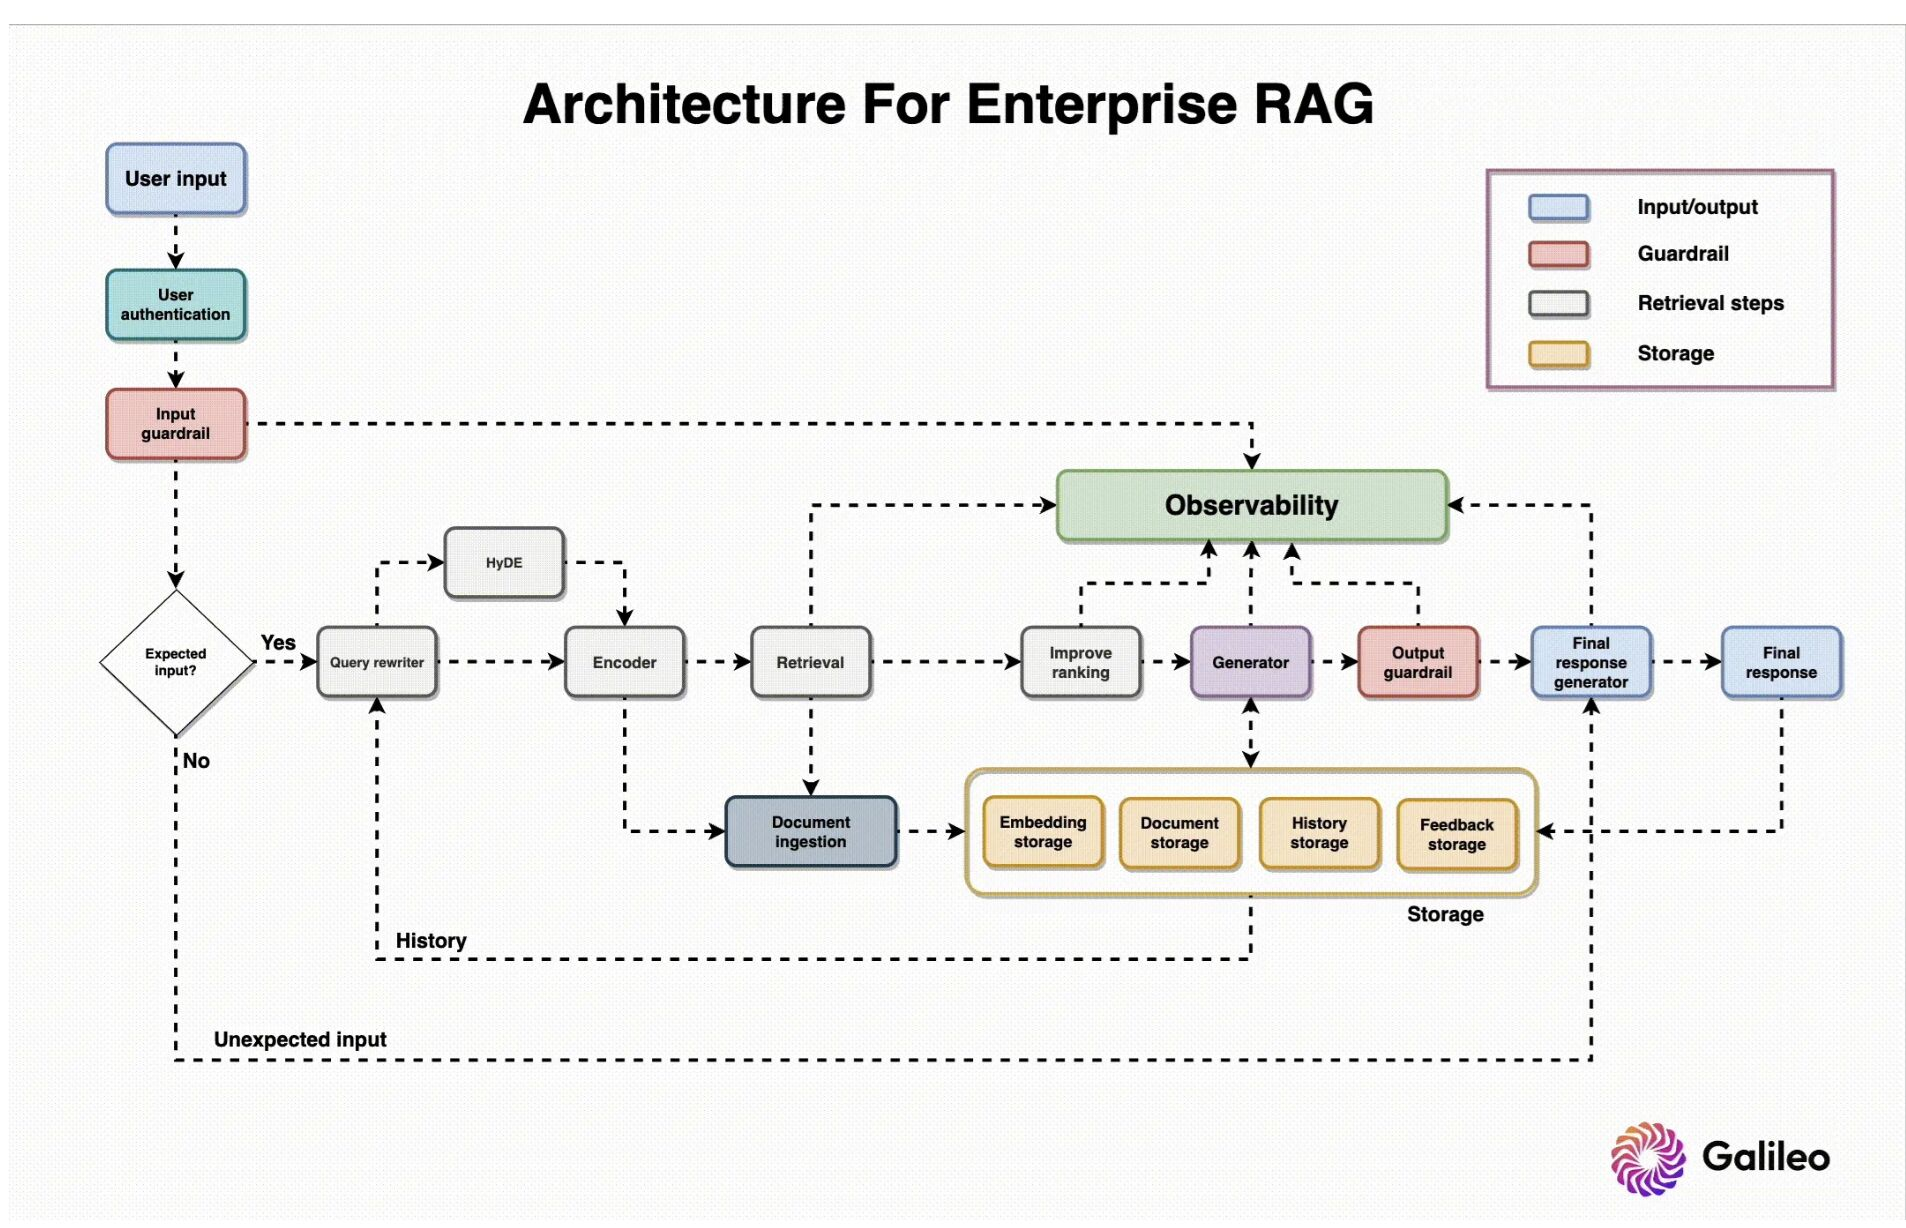
\includegraphics[width=0.8\linewidth,keepaspectratio]{rag63}
		
		{\tiny (Ref: LinkedIn post by Sarthak Rastogi)}
        \end{center}	

\end{frame}


%%%%%%%%%%%%%%%%%%%%%%%%%%%%%%%%%%%%%%%%%%%%%%%%%%%%%%%%%%%%%%%%%%%%%%%%%%%%%%%%%%
\begin{frame}[fragile]\frametitle{}
\begin{center}
{\Large Vector DB in Production}

{\tiny (Ref: LinkedIn post by Nirant Kasliwal)}
\end{center}
\end{frame}


%%%%%%%%%%%%%%%%%%%%%%%%%%%%%%%%%%%%%%%%%%%%%%%%%%%%%%%%%%%%%%%%%%%%%%%%%%%%%%%%%%
\begin{frame}[fragile]\frametitle{The Problem}
\begin{itemize}
    \item Vector search choices often spark endless technical debates.
    \item Teams struggle to balance speed, quality, and cost.
    \item Poor decisions stem from unclear priorities.
\end{itemize}
\end{frame}

%%%%%%%%%%%%%%%%%%%%%%%%%%%%%%%%%%%%%%%%%%%%%%%%%%%%%%%%%%%%%%%%%%%%%%%%%%%%%%%%%%
\begin{frame}[fragile]\frametitle{The Tradeoff Triangle}
\begin{itemize}
    \item Vector search is a balance of:
    \begin{itemize}
        \item Speed (low latency)
        \item Quality (high recall)
        \item Cost (infrastructure)
    \end{itemize}
    \item You can only optimize two; the third will suffer.
    \item Overpromising all three leads to failure.
\end{itemize}
\end{frame}

%%%%%%%%%%%%%%%%%%%%%%%%%%%%%%%%%%%%%%%%%%%%%%%%%%%%%%%%%%%%%%%%%%%%%%%%%%%%%%%%%%
\begin{frame}[fragile]\frametitle{Why a Decision Framework Helps}
\begin{itemize}
    \item Avoids circular discussions.
    \item Focuses on business needs, not technical preferences.
    \item Saves time and clarifies tradeoffs.
\end{itemize}
\end{frame}

%%%%%%%%%%%%%%%%%%%%%%%%%%%%%%%%%%%%%%%%%%%%%%%%%%%%%%%%%%%%%%%%%%%%%%%%%%%%%%%%%%
\begin{frame}[fragile]\frametitle{Concrete Questions Over Abstract Debates}
\begin{itemize}
    \item Is cost a hard constraint?
    \item Do we need latency under 50ms?
    \item What recall can users actually perceive?
\end{itemize}
\end{frame}

%%%%%%%%%%%%%%%%%%%%%%%%%%%%%%%%%%%%%%%%%%%%%%%%%%%%%%%%%%%%%%%%%%%%%%%%%%%%%%%%%%
\begin{frame}[fragile]\frametitle{A Real-World Example}
\begin{itemize}
    \item Product team wanted ``Google recall'' + ``Stripe latency'' + startup budget.
    \item Framework helped align on priorities.
    \item Solution: quantized index optimized for user-impacting metrics.
\end{itemize}
\end{frame}

%%%%%%%%%%%%%%%%%%%%%%%%%%%%%%%%%%%%%%%%%%%%%%%%%%%%%%%%%%%%%%%%%%%%%%%%%%%%%%%%%%
\begin{frame}[fragile]\frametitle{Vector Search = Navigation}
\begin{itemize}
    \item Optimization is like choosing a GPS route.
    \item Fastest isn’t always best—consider tolls and risk.
    \item Decision tree guides you to the best compromise.
\end{itemize}
\end{frame}

%%%%%%%%%%%%%%%%%%%%%%%%%%%%%%%%%%%%%%%%%%%%%%%%%%%%%%%%%%%%%%%%%%%%%%%%%%%%%%%%%%
\begin{frame}[fragile]\frametitle{Vector Db Descion Tree}
		\begin{center}
		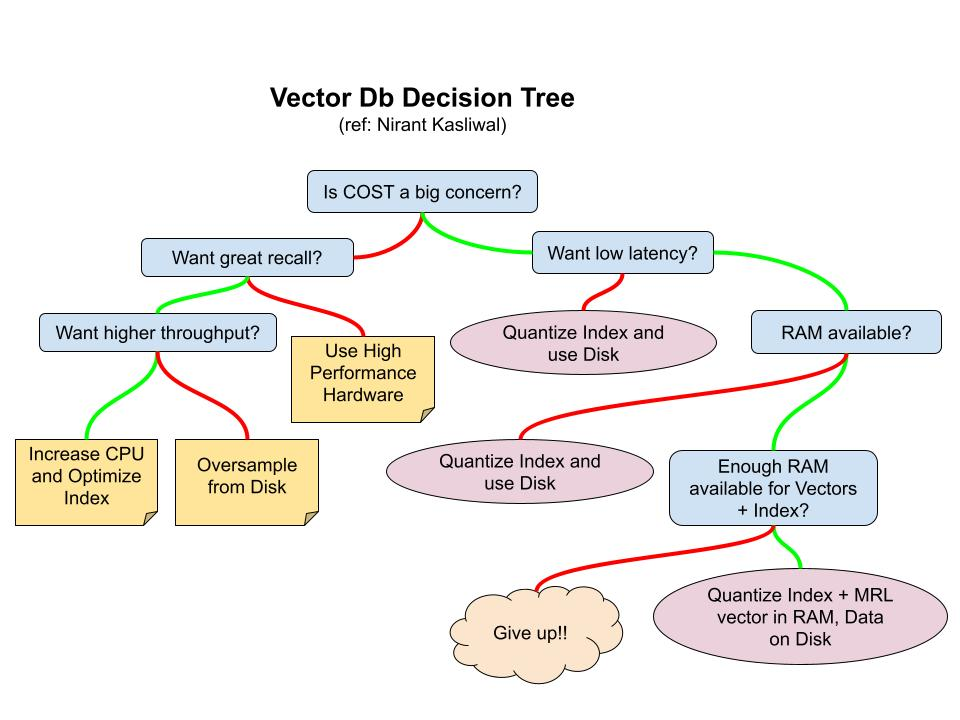
\includegraphics[width=0.8\linewidth,keepaspectratio]{rag38}
		\end{center}
\end{frame}

%%%%%%%%%%%%%%%%%%%%%%%%%%%%%%%%%%%%%%%%%%%%%%%%%%%%%%%%%%%%%%%%%%%%%%%%%%%%%%%%%%
\begin{frame}[fragile]\frametitle{Key Takeaway}
\begin{itemize}
    \item Use structured questions to steer tradeoffs.
    \item Let business goals—not tech idealism—drive choices.
    \item This framework turns friction into clarity.
\end{itemize}
\end{frame}

%%%%%%%%%%%%%%%%%%%%%%%%%%%%%%%%%%%%%%%%%%%%%%%%%%%%%%%%%%%%%%%%%%%%%%%%%%%%%%%%%%
\begin{frame}[fragile]\frametitle{}
\begin{center}
{\Large Embedding Model}

\end{center}
\end{frame}

%%%%%%%%%%%%%%%%%%%%%%%%%%%%%%%%%%%%%%%%%%%%%%%%%%%%%%%%%%%
\begin{frame}[fragile]\frametitle{What is RAG?}
    \begin{itemize}
        \item RAG augments LLM responses with context retrieved from a vector store.
        \item Similarity search retrieves relevant documents via query-document embedding comparisons.
        \item Embedding quality critically impacts retrieval and overall RAG performance.
        \item Choice of embedding model directly influences LLM response quality.
    \end{itemize}
\end{frame}

%%%%%%%%%%%%%%%%%%%%%%%%%%%%%%%%%%%%%%%%%%%%%%%%%%%%%%%%%%%
\begin{frame}[fragile]\frametitle{Choosing an Embedding Model}
    \begin{itemize}
        \item Use MTEB leaderboard to assess embedding model performance.
        \item MTEB ranks models across diverse NLP tasks for comprehensive evaluation.
        \item However, top rank does not always imply best fit for your use case.
		\item Which Embedding dimension? As much as you can, though more meaningful, can make search slwoer
		\item Most models don't allow size change so be sure at first.
    \end{itemize}
\end{frame}

%%%%%%%%%%%%%%%%%%%%%%%%%%%%%%%%%%%%%%%%%%%%%%%%%%%%%%%%%%%%%%%%%%%%%%%%%%%%%%%%%%
\begin{frame}[fragile]\frametitle{MTEB Leaderboard}
Hugging Face MTEB (Massive Text Embedding Benchmark) leaderboard, as shown below:

		\begin{center}
		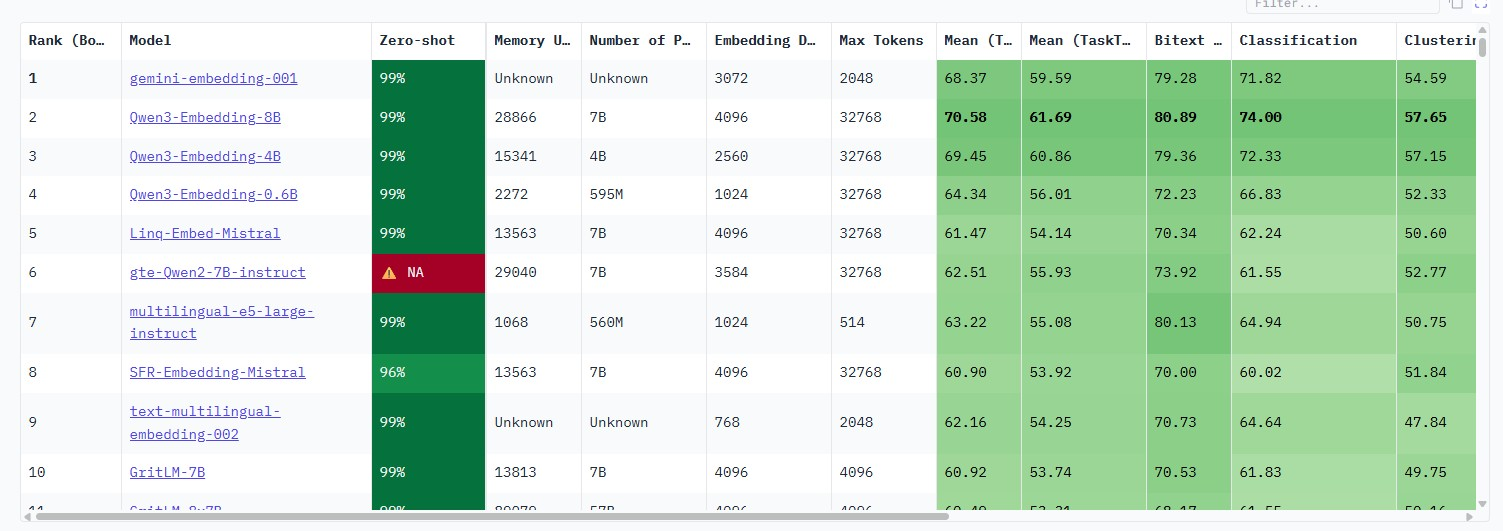
\includegraphics[width=\linewidth,keepaspectratio]{llm169}
		
		{\tiny (Ref: https://huggingface.co/spaces/mteb/leaderboard on 1 July 2025)}
		
		\end{center}


\end{frame}


%%%%%%%%%%%%%%%%%%%%%%%%%%%%%%%%%%%%%%%%%%%%%%%%%%%%%%%%%%%
\begin{frame}[fragile]\frametitle{Understanding the MTEB Leaderboard}
    \begin{itemize}
        \item Hosted on Hugging Face to benchmark embedding models.
        \item Covers tasks like classification, clustering, retrieval, STS (Semantic Texutal Similarity), summarization.
		\item STS focuses on measuring the semantic similarity between sentence pairs, while retrieval aims to find relevant documents from a corpus given a query
        \item Enables holistic model comparison across varied NLP scenarios.
    \end{itemize}
\end{frame}

%%%%%%%%%%%%%%%%%%%%%%%%%%%%%%%%%%%%%%%%%%%%%%%%%%%%%%%%%%%
\begin{frame}[fragile]\frametitle{Factors in Model Selection}
    \begin{itemize}
        \item Evaluate performance on tasks relevant to your use case.
        \item Consider compute requirements and inference speed.
        \item Prefer domain-specific models for specialized applications.
        \item Test models using your actual data for best alignment.
    \end{itemize}
\end{frame}

%%%%%%%%%%%%%%%%%%%%%%%%%%%%%%%%%%%%%%%%%%%%%%%%%%%%%%%%%%
\begin{frame}[fragile]\frametitle{Domain-Specific Models}
    \begin{itemize}
        \item \textbf{Medicine}: PubMedBERT, BioLORD for clinical and biomedical texts.
        \item \textbf{Finance}: Investopedia, Voyage, BGE Financial Matryoshka.
        \item \textbf{Law}: Legal-specific models for legal research and analysis.
        \item \textbf{Code}: CodeBERT, GraphCodeBERT for programming-related tasks.
        \item \textbf{Math}: Math Similarity Model for mathematical expressions.
    \end{itemize}
\end{frame}

%%%%%%%%%%%%%%%%%%%%%%%%%%%%%%%%%%%%%%%%%%%%%%%%%%%%%%%%%%%
\begin{frame}[fragile]\frametitle{Models for Other Languages}
    \begin{itemize}
        \item \textbf{Japanese}: RoSEtta-base-ja
        \item \textbf{Korean}: KoSimCSE-roberta
        \item \textbf{Chinese}: GTE-Qwen2-7B-instruct
        \item \textbf{French}: Sentence-Camembert-large
        \item \textbf{Arabic}: Arabic-STS-Matryoshka
    \end{itemize}
\end{frame}

%%%%%%%%%%%%%%%%%%%%%%%%%%%%%%%%%%%%%%%%%%%%%%%%%%%%%%%%%%%%%%%%%%%%%%%%%%%%%%%%%%
\begin{frame}[fragile]\frametitle{}
\begin{center}
{\Large LLM/RAG in Production}

{\tiny (Ref:  Shipping LLM: Addressing Production Challenges - Venkatesh \& Suman)}
\end{center}
\end{frame}

%%%%%%%%%%%%%%%%%%%%%%%%%%%%%%%%%%%%%%%%%%%%%%%%%%%%%%%%%%%
\begin{frame}[fragile]\frametitle{Factors to Consider Before LLM/RAG Deployment}
  \begin{itemize}
    \item Evaluate metrics before putting LLMs or RAG into production.
    \item Consider cost, latency, and throughput during model selection.
    \item Choose between open-source vs. proprietary models.
    \item Ensure high response quality and relevance.
    \item Establish a unified framework for evaluating production readiness.
  \end{itemize}
\end{frame}

%%%%%%%%%%%%%%%%%%%%%%%%%%%%%%%%%%%%%%%%%%%%%%%%%%%%%%%%%%%
\begin{frame}[fragile]\frametitle{Four Major Industrial Focus Areas}
  \begin{itemize}
    \item Document processing and information extraction.
    \item Knowledge base and question answering systems.
    \item Domain-specific conversational agents (e.g., logistics, customer support).
    \item Workflow automation using generative AI (e.g., email handling).
    \item These are not exhaustive but reflect current industry trends.
  \end{itemize}
  
	\begin{center}
	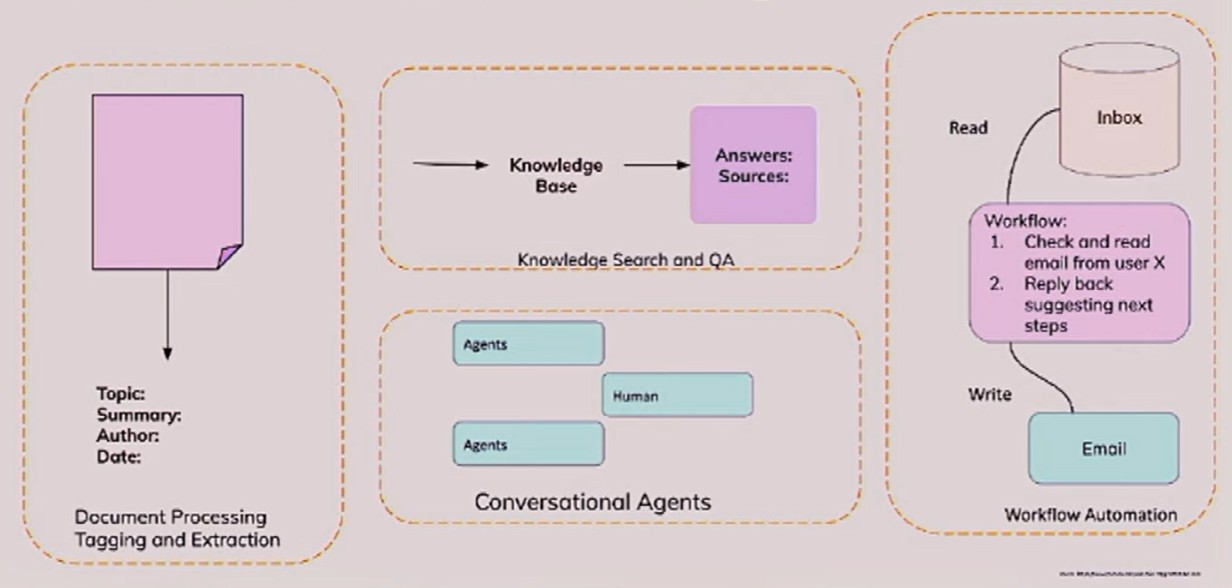
\includegraphics[width=0.8\linewidth,keepaspectratio]{llm170}
	
	{\tiny (Ref: Shipping LLM: Addressing Production Challenges - Venkatesh \& Suman)}
	\end{center}
  
\end{frame}

%%%%%%%%%%%%%%%%%%%%%%%%%%%%%%%%%%%%%%%%%%%%%%%%%%%%%%%%%%%
\begin{frame}[fragile]\frametitle{RAG Pipeline Overview}
  \begin{itemize}
    \item Data ingestion: chunking and embedding documents.
    \item Data retrieval: semantic search from vector databases.
    \item Data synthesis: LLM generates answer using retrieved chunks.
    \item Pipeline involves multiple tightly coupled components.
    \item Output: curated, context-aware response to user query.
  \end{itemize}
  
	\begin{center}
	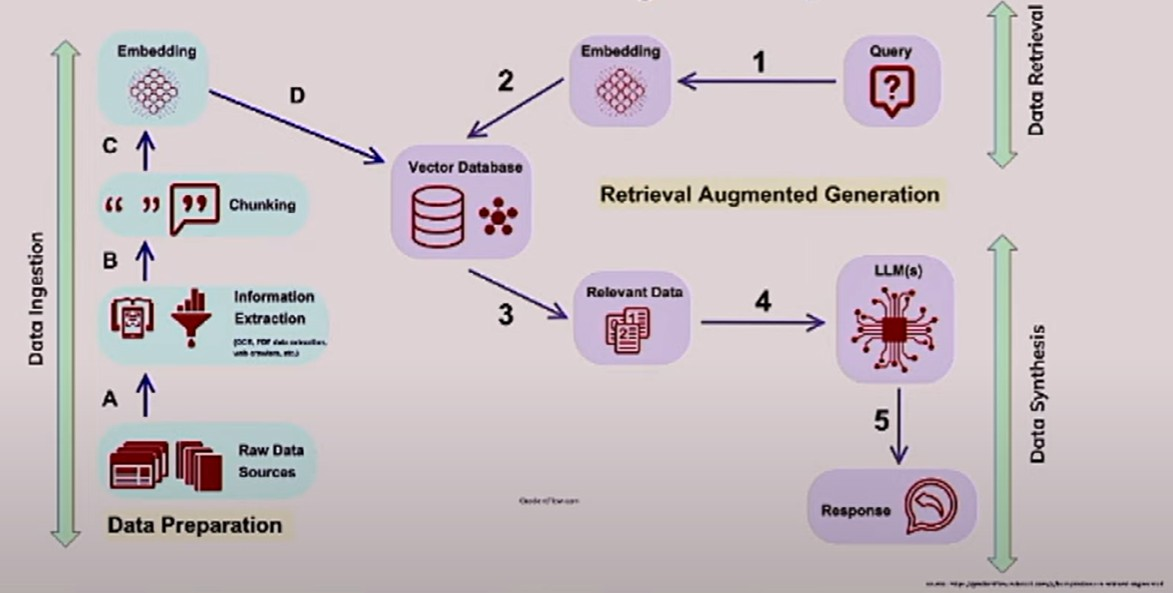
\includegraphics[width=0.8\linewidth,keepaspectratio]{llm171}
	
	{\tiny (Ref: Shipping LLM: Addressing Production Challenges - Venkatesh \& Suman)}
	\end{center}  
\end{frame}

%%%%%%%%%%%%%%%%%%%%%%%%%%%%%%%%%%%%%%%%%%%%%%%%%%%%%%%%%%%
\begin{frame}[fragile]\frametitle{Production Challenges in RAG Systems}
  \begin{itemize}
    \item Building a demo is easier than productionizing RAG.
    \item Ensure high-quality responses with minimal hallucinations.
    \item Evaluate and compare different RAG approaches.
    \item Validate sub-pipeline performance independently.
    \item Continuously monitor system via ML Ops practices.
  \end{itemize}
\end{frame}

%%%%%%%%%%%%%%%%%%%%%%%%%%%%%%%%%%%%%%%%%%%%%%%%%%%%%%%%%%%
\begin{frame}[fragile]\frametitle{Retrieval Issues in RAG}
  \begin{itemize}
    \item \textbf{Low precision}: irrelevant chunks retrieved (e.g., Banur example).
    \item \textbf{Low recall}: important chunks may be missed.
    \item Retrieval quality directly impacts final response relevance.
    \item Fixing retrieval quality is crucial before tuning generation.
    \item Retrieval performance is often the primary bottleneck.
  \end{itemize}
\end{frame}

%%%%%%%%%%%%%%%%%%%%%%%%%%%%%%%%%%%%%%%%%%%%%%%%%%%%%%%%%%%
\begin{frame}[fragile]\frametitle{LLM Generation Issues in RAG}
  \begin{itemize}
    \item \textbf{Hallucination}: generating incorrect or fabricated facts.
    \item \textbf{Irrelevance}: off-topic responses from the LLM.
    \item \textbf{Toxicity}: potentially offensive content.
    \item Importance of implementing guardrails and filters.
    \item Regular evaluation and reinforcement needed for safe deployment.
  \end{itemize}
\end{frame}

%%%%%%%%%%%%%%%%%%%%%%%%%%%%%%%%%%%%%%%%%%%%%%%%%%%%%%%%%%%
\begin{frame}[fragile]\frametitle{Evaluation Metrics for Retrieval}
  \begin{itemize}
    \item \textbf{Context recall}: fraction of relevant chunks retrieved.
    \item \textbf{Context precision}: fraction of retrieved chunks that are relevant.
    \item \textbf{Hit rate}: binary metric of whether any relevant chunk was retrieved.
    \item \textbf{MRR (Mean Reciprocal Rank)}: rank of first relevant item.
    \item Helps quantify retrieval pipeline effectiveness.
  \end{itemize}

	\begin{center}
	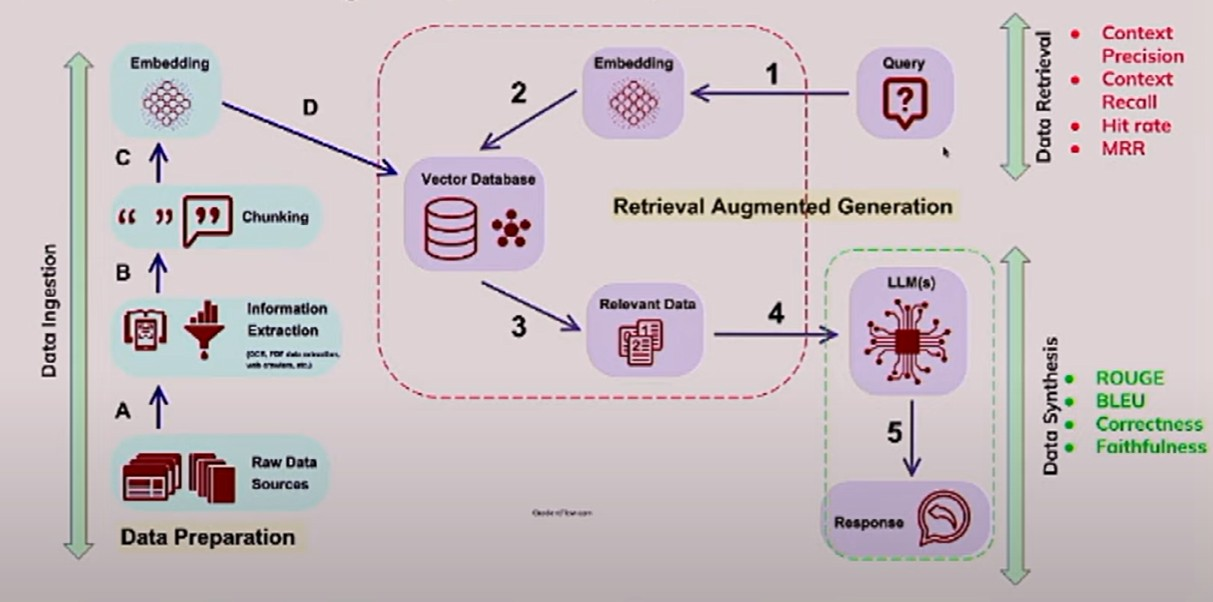
\includegraphics[width=0.8\linewidth,keepaspectratio]{llm172}
	
	{\tiny (Ref: Shipping LLM: Addressing Production Challenges - Venkatesh \& Suman)}
	\end{center}   
\end{frame}

%%%%%%%%%%%%%%%%%%%%%%%%%%%%%%%%%%%%%%%%%%%%%%%%%%%%%%%%%%%
\begin{frame}[fragile]\frametitle{Evaluation Metrics for Retrieval}

	\begin{center}
	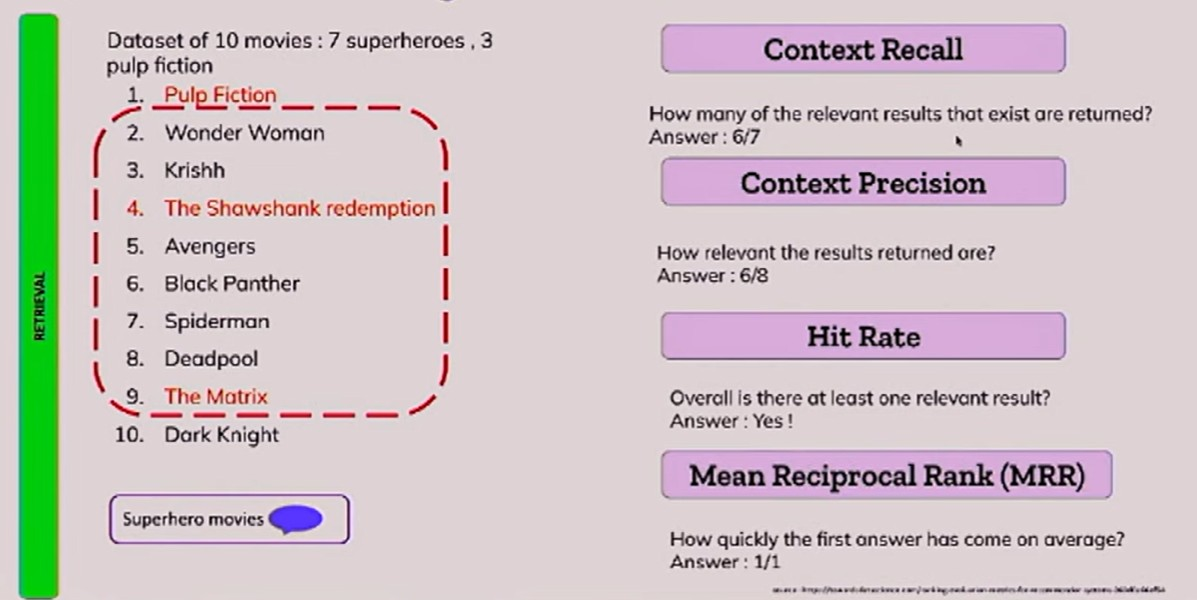
\includegraphics[width=\linewidth,keepaspectratio]{llm173}
	
	{\tiny (Ref: Shipping LLM: Addressing Production Challenges - Venkatesh \& Suman)}
	\end{center}   
\end{frame}


%%%%%%%%%%%%%%%%%%%%%%%%%%%%%%%%%%%%%%%%%%%%%%%%%%%%%%%%%%%
\begin{frame}[fragile]\frametitle{Evaluation Metrics for Generation}
  \begin{itemize}
    \item \textbf{ROUGE}: overlap of n-grams for summarization accuracy.
    \item \textbf{BLEU}: word overlap between generated and reference text.
    \item \textbf{METEOR}: synonym-aware overlap evaluation.
    \item \textbf{LLM metrics}: faithfulness, correctness, and toxicity.
    \item Enables robust scoring of output text quality.
  \end{itemize}
\end{frame}

%%%%%%%%%%%%%%%%%%%%%%%%%%%%%%%%%%%%%%%%%%%%%%%%%%%%%%%%%%%
\begin{frame}[fragile]\frametitle{Evaluation Metrics for Generation}

	\begin{center}
	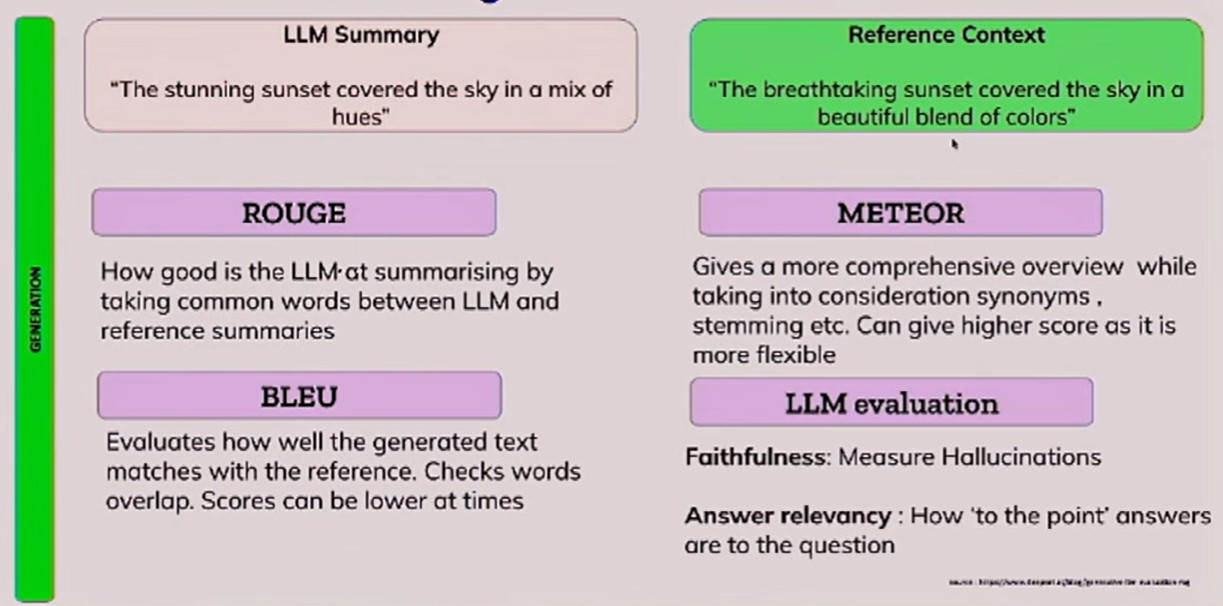
\includegraphics[width=\linewidth,keepaspectratio]{llm174}
	
	{\tiny (Ref: Shipping LLM: Addressing Production Challenges - Venkatesh \& Suman)}
	\end{center}   
\end{frame}

%%%%%%%%%%%%%%%%%%%%%%%%%%%%%%%%%%%%%%%%%%%%%%%%%%%%%%%%%%%
\begin{frame}[fragile]\frametitle{Evaluation Metrics for Frameworks}

	\begin{center}
	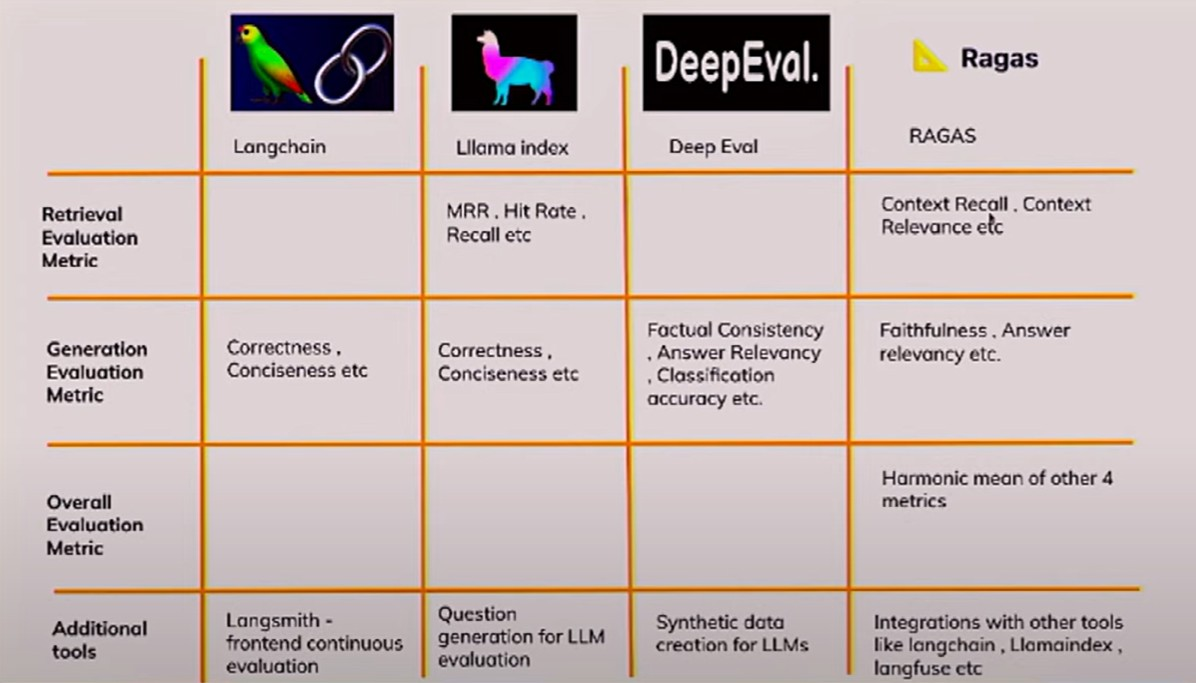
\includegraphics[width=\linewidth,keepaspectratio]{llm175}
	
	{\tiny (Ref: Shipping LLM: Addressing Production Challenges - Venkatesh \& Suman)}
	\end{center}   
\end{frame}

%%%%%%%%%%%%%%%%%%%%%%%%%%%%%%%%%%%%%%%%%%%%%%%%%%%%%%%%%%%
\begin{frame}[fragile]\frametitle{End-to-End Evaluation: RAG Triad}
  \begin{itemize}
    \item \textbf{Answer relevance}: does output match the query intent?
    \item \textbf{Context relevance}: are retrieved chunks relevant?
    \item \textbf{Groundedness}: is answer supported by retrieved content?
    \item Context relevance is most critical for response quality.
    \item Use TrueLens or similar tools for triad analysis.
  \end{itemize}
  
	\begin{center}
	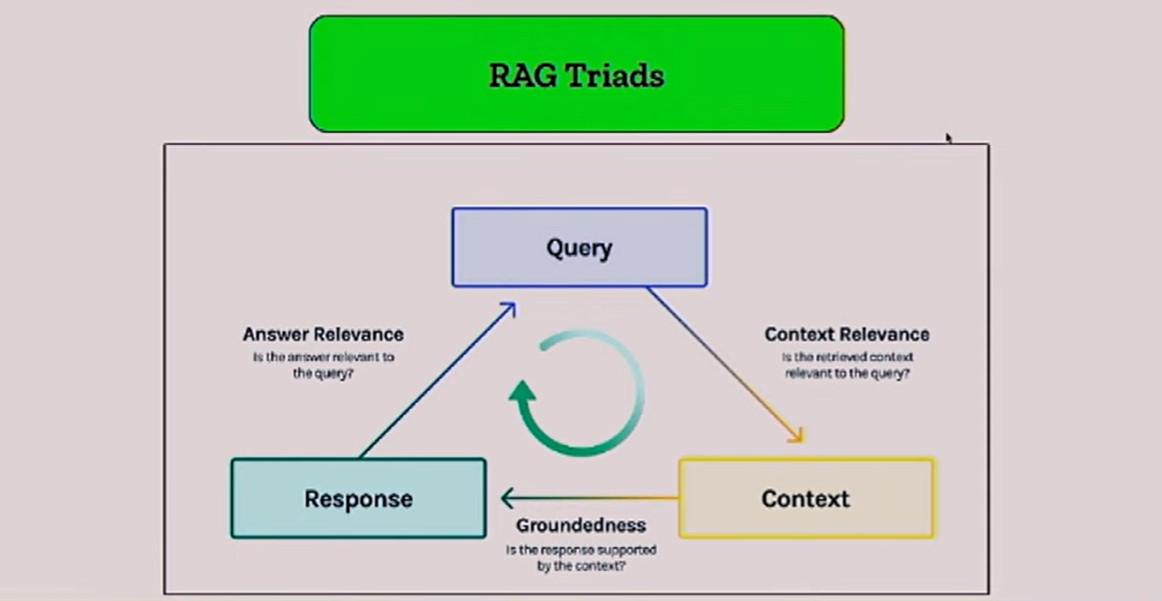
\includegraphics[width=0.8\linewidth,keepaspectratio]{llm176}
	
	{\tiny (Ref: Shipping LLM: Addressing Production Challenges - Venkatesh \& Suman)}
	\end{center}     
\end{frame}

%%%%%%%%%%%%%%%%%%%%%%%%%%%%%%%%%%%%%%%%%%%%%%%%%%%%%%%%%%%
\begin{frame}[fragile]\frametitle{Sample Two Columns Slide}
% \begin{columns}
    % \begin{column}[T]{0.5\linewidth}
		\begin{center}
		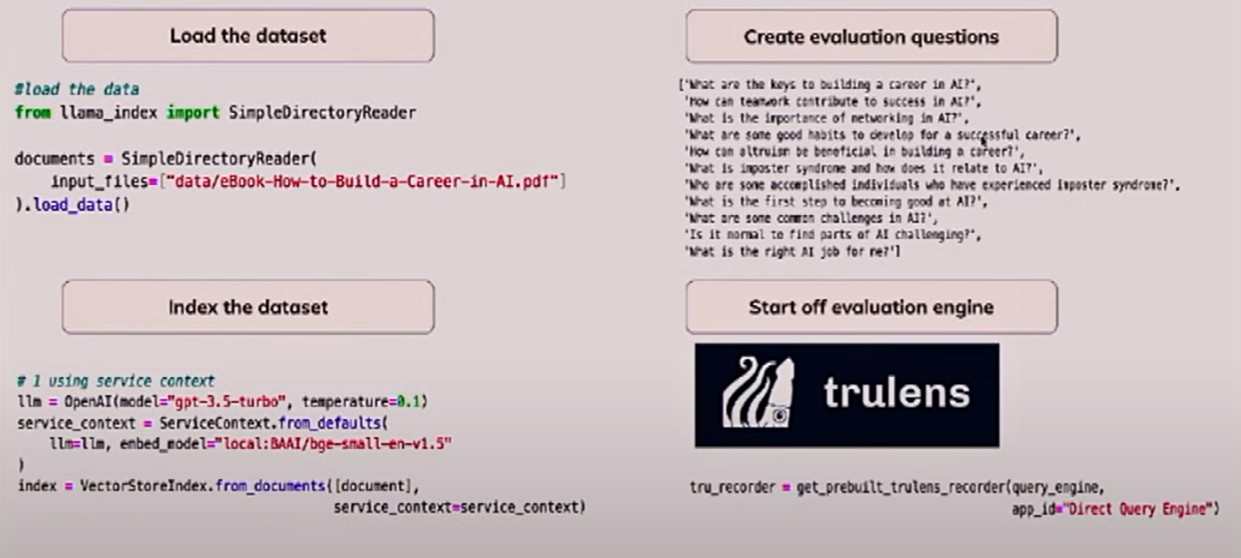
\includegraphics[width=0.7\linewidth,keepaspectratio]{llm177}
		\end{center}  
    % \end{column}
    % \begin{column}[T]{0.5\linewidth}
		\begin{center}
		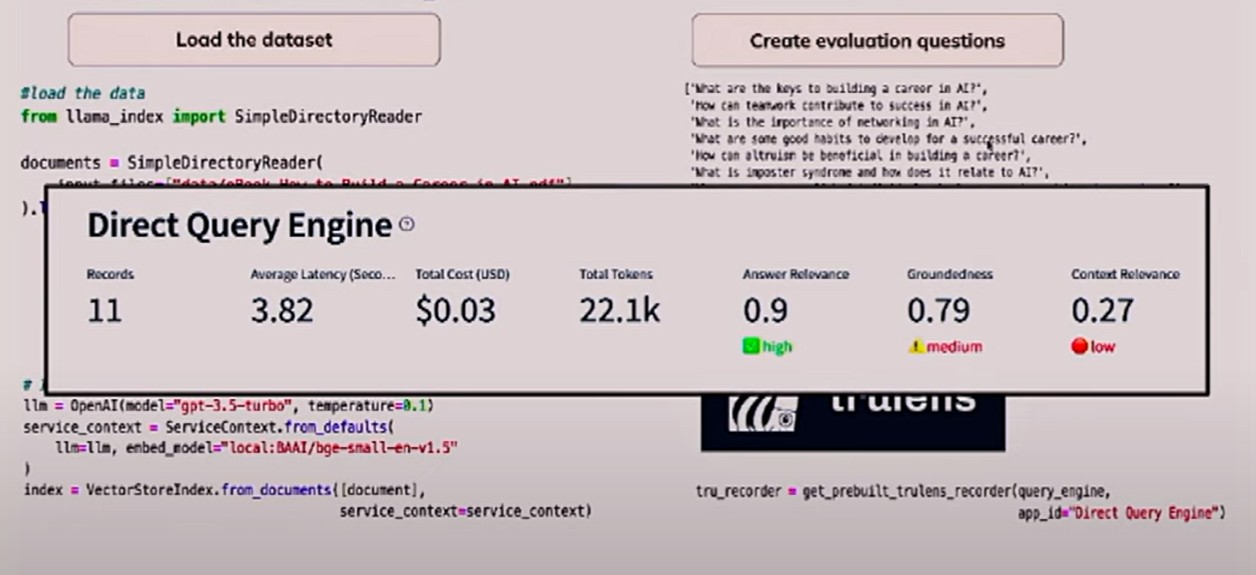
\includegraphics[width=0.7\linewidth,keepaspectratio]{llm178}
		\end{center}  
    % \end{column}
  % \end{columns}
  
	{\tiny (Ref: Shipping LLM: Addressing Production Challenges - Venkatesh \& Suman)}
  
\end{frame}


%%%%%%%%%%%%%%%%%%%%%%%%%%%%%%%%%%%%%%%%%%%%%%%%%%%%%%%%%%%
\begin{frame}[fragile]\frametitle{Improving RAG: Optimization Techniques}
  \begin{itemize}
    \item \textbf{Sentence Window Retrieval}: retrieve context with surrounding sentences.
    \item Enhances context richness, increasing relevance and groundedness.
    \item \textbf{Auto-merging Retrieval}: combine overlapping chunks for completeness.
    \item Better context results in higher-quality LLM responses.
    \item Evaluate and tune using metrics before production.
  \end{itemize}
\end{frame}

%%%%%%%%%%%%%%%%%%%%%%%%%%%%%%%%%%%%%%%%%%%%%%%%%%%%%%%%%%%
\begin{frame}[fragile]\frametitle{Sentence Window Retrieval}

	\begin{center}
	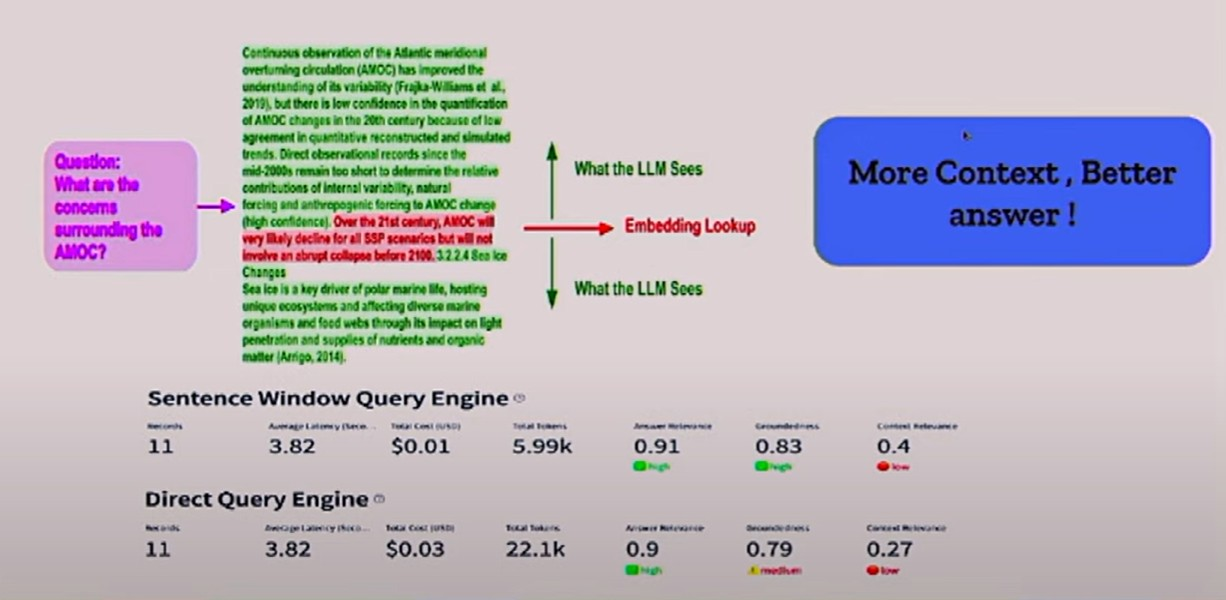
\includegraphics[width=\linewidth,keepaspectratio]{llm179}
	
	{\tiny (Ref: Shipping LLM: Addressing Production Challenges - Venkatesh \& Suman)}
	\end{center}   
\end{frame}


%%%%%%%%%%%%%%%%%%%%%%%%%%%%%%%%%%%%%%%%%%%%%%%%%%%%%%%%%%
\begin{frame}[fragile]\frametitle{Auto-merging Retrieval}

	\begin{center}
	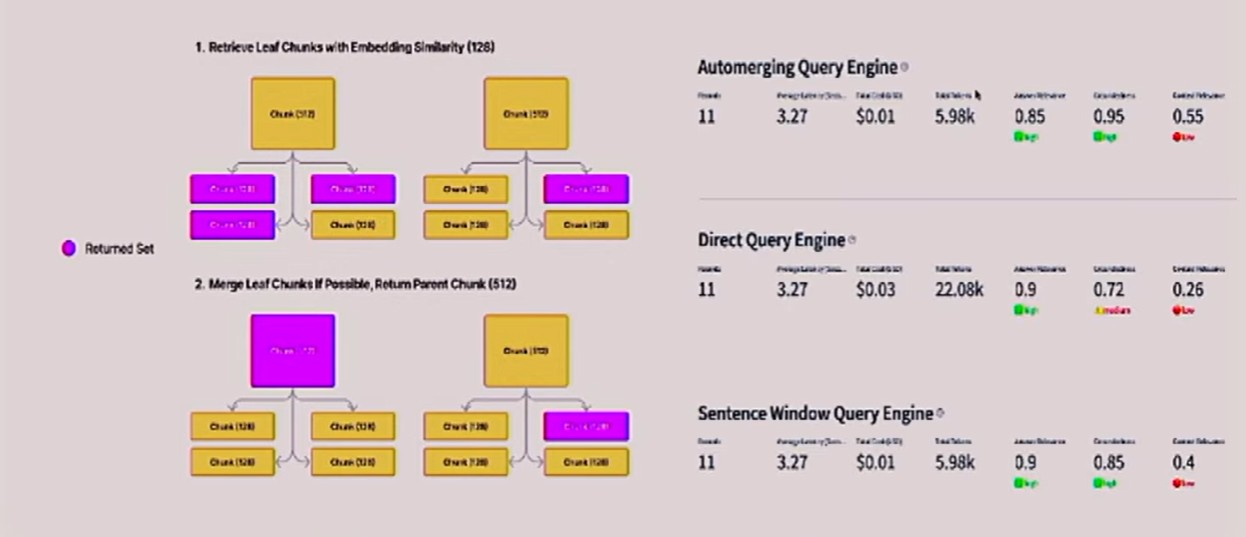
\includegraphics[width=\linewidth,keepaspectratio]{llm180}
	
	{\tiny (Ref: Shipping LLM: Addressing Production Challenges - Venkatesh \& Suman)}
	\end{center}   
\end{frame}

%%%%%%%%%%%%%%%%%%%%%%%%%%%%%%%%%%%%%%%%%%%%%%%%%%%%%%%%%%
\begin{frame}[fragile]\frametitle{More \ldots}

	\begin{center}
	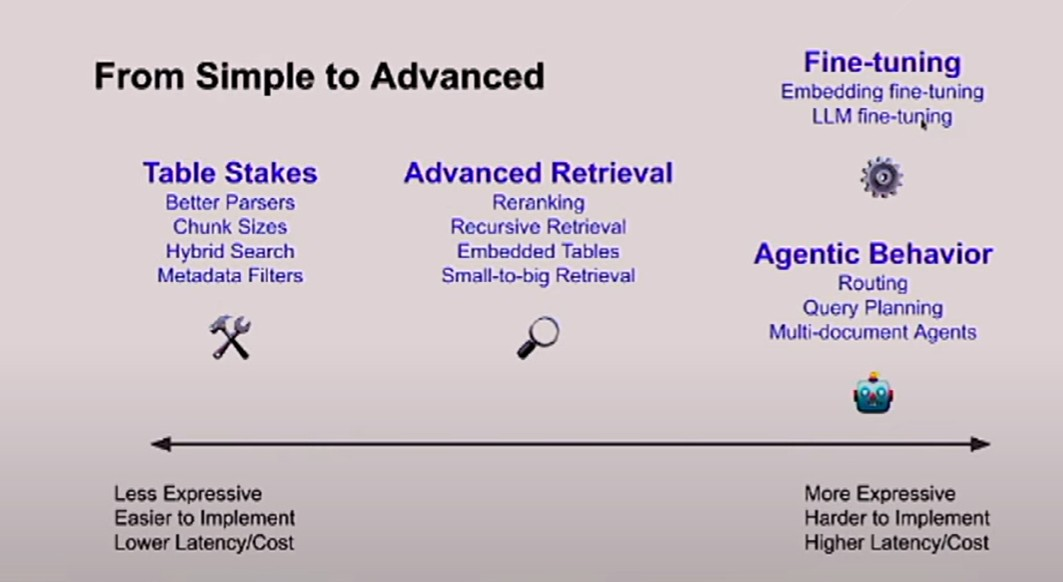
\includegraphics[width=\linewidth,keepaspectratio]{llm181}
	
	{\tiny (Ref: Shipping LLM: Addressing Production Challenges - Venkatesh \& Suman)}
	\end{center}   
\end{frame}



%%%%%%%%%%%%%%%%%%%%%%%%%%%%%%%%%%%%%%%%%%%%%%%%%%%%%%%%%%
\begin{frame}[fragile]\frametitle{Evaluation Frameworks and Tools}
  \begin{itemize}
    \item Popular frameworks: LangChain, LlamaIndex, TruLens, RAGAS.
    \item Each offers tools for retrieval and generation evaluation.
    \item Some provide full support for RAG Triad scoring.
    \item Choose tools based on needs (e.g., preference for RAGAS).
    \item Experiment with multiple frameworks to validate performance.
  \end{itemize}
\end{frame}

%%%%%%%%%%%%%%%%%%%%%%%%%%%%%%%%%%%%%%%%%%%%%%%%%%%%%%%%%%%
\begin{frame}[fragile]\frametitle{More \ldots}

	\begin{center}
	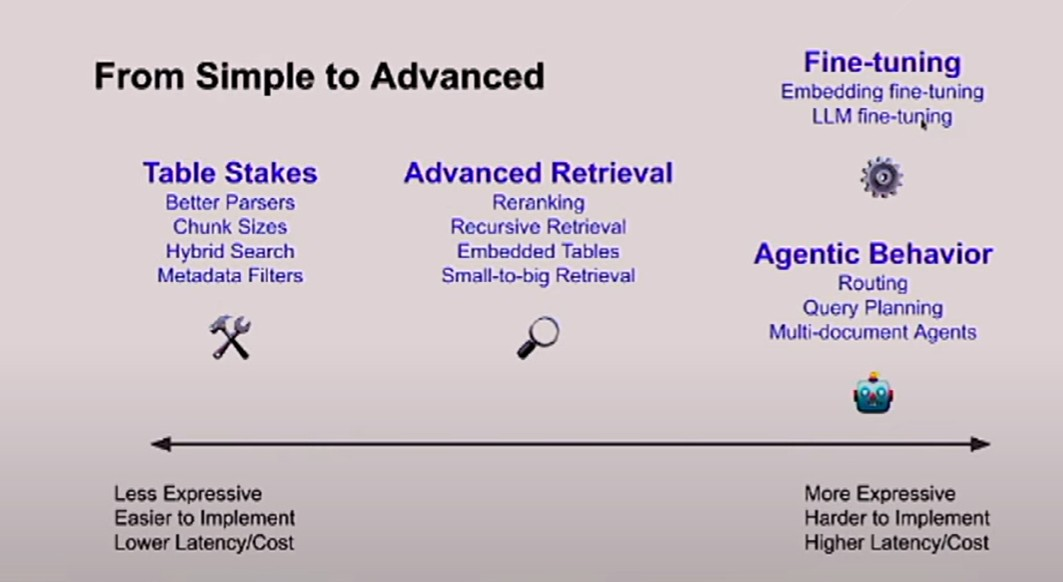
\includegraphics[width=\linewidth,keepaspectratio]{llm181}
	
	{\tiny (Ref: Shipping LLM: Addressing Production Challenges - Venkatesh \& Suman)}
	\end{center}   
\end{frame}

%%%%%%%%%%%%%%%%%%%%%%%%%%%%%%%%%%%%%%%%%%%%%%%%%%%%%%%%%%%
\begin{frame}[fragile]\frametitle{Cost Analysis Components}
      \begin{itemize}
	\item Initial Setup \& Inference: Model storage and prediction costs
	\item Maintenance: Fine-tuning, training, and data labeling expenses
	\item Associated Costs: CO2 emissions, carbon footprint impact
	\item Human Resources: Training costs and specialized talent acquisition
	\item Daily usage can exceed AWS costs for extensive applications
	  \end{itemize}
	  
	\begin{center}
	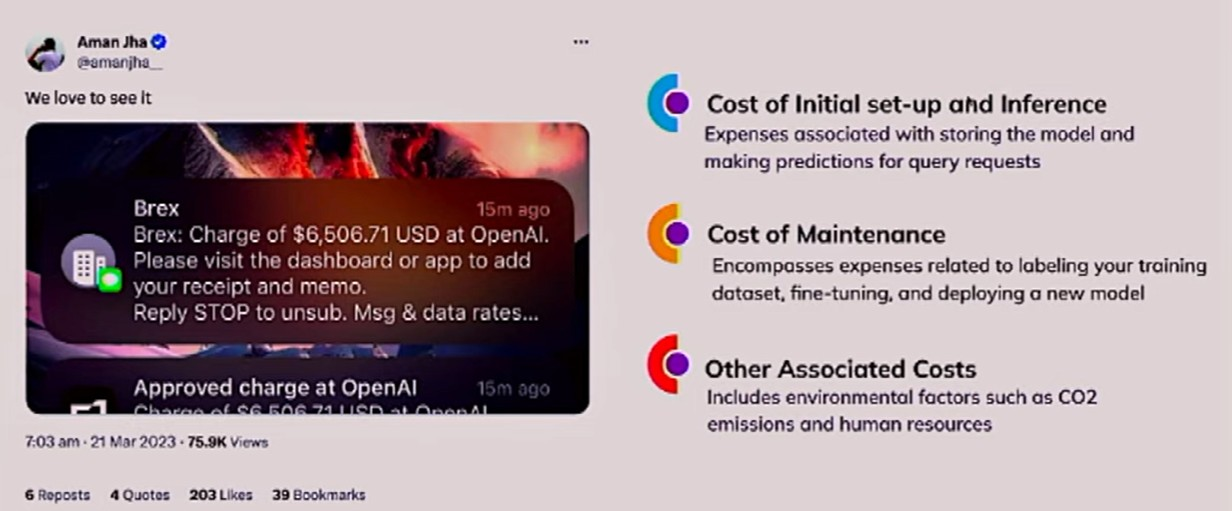
\includegraphics[width=\linewidth,keepaspectratio]{llm182}
	
	{\tiny (Ref: Shipping LLM: Addressing Production Challenges - Venkatesh \& Suman)}
	\end{center}   	  
\end{frame}

%%%%%%%%%%%%%%%%%%%%%%%%%%%%%%%%%%%%%%%%%%%%%%%%%%%%%%%%%%%
\begin{frame}[fragile]\frametitle{Third-Party API vs On-Premise Hosting}
      \begin{itemize}
	\item OpenAI APIs: Separate costs for input tokens, output tokens, per-request
	\item Local hosting viable for 3-7 billion parameter models with decent hardware
	\item Cloud instances: \$0.6 to \$45 per hour for large models (30B-70B parameters)
	\item A800 Nvidia GPUs: Up to 640GB GPU RAM for massive models
	\item Decision based on parameter count and cost comparison analysis
	  \end{itemize}

	\begin{center}
	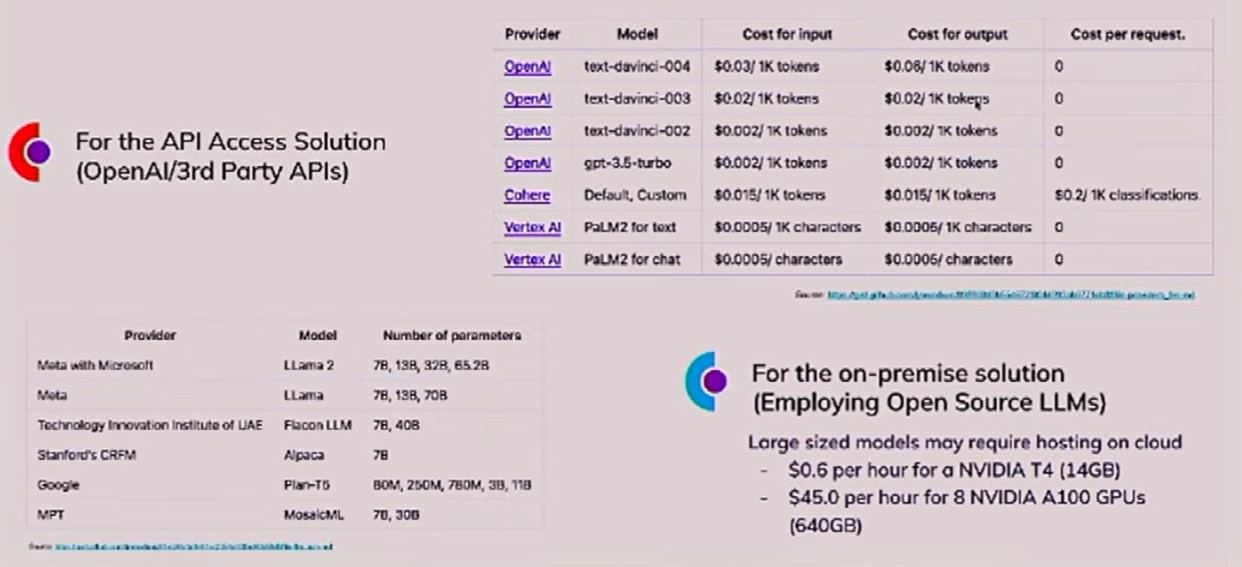
\includegraphics[width=0.8\linewidth,keepaspectratio]{llm183}
	
	{\tiny (Ref: Shipping LLM: Addressing Production Challenges - Venkatesh \& Suman)}
	\end{center}   
\end{frame}

%%%%%%%%%%%%%%%%%%%%%%%%%%%%%%%%%%%%%%%%%%%%%%%%%%%%%%%%%%%
\begin{frame}[fragile]\frametitle{Maintenance Cost Structures}
      \begin{itemize}
	\item Vertex AI AutoML: Upload, training, deployment, prediction costs
	\item OpenAI: Training cost plus input/output usage fees
	\item Data labeling: Third-party platforms or human annotators
	\item Fine-tuning expenses vary by model size and training duration
	\item Free data upload up to first 1000 pages in some platforms
	  \end{itemize}


\end{frame}

%%%%%%%%%%%%%%%%%%%%%%%%%%%%%%%%%%%%%%%%%%%%%%%%%%%%%%%%%%%
\begin{frame}[fragile]\frametitle{Maintenance Cost Structures}

	\begin{center}
	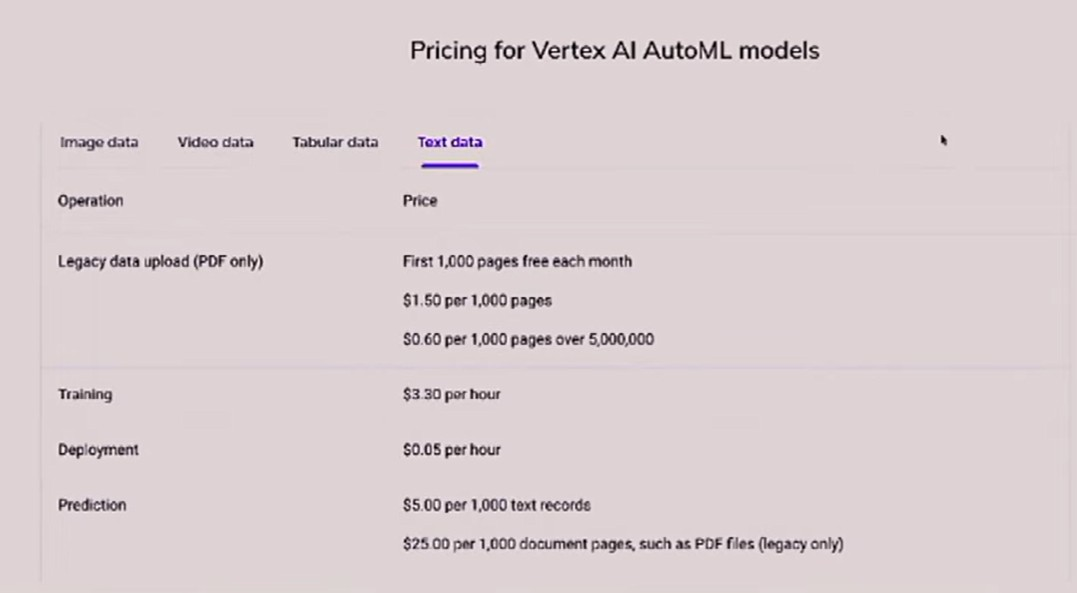
\includegraphics[width=0.7\linewidth,keepaspectratio]{llm184}
	
	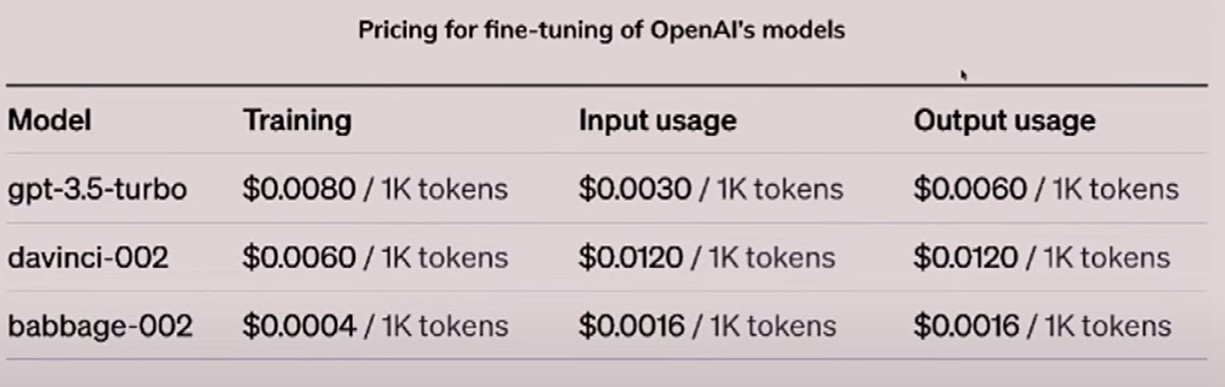
\includegraphics[width=0.7\linewidth,keepaspectratio]{llm185}

	{\tiny (Ref: Shipping LLM: Addressing Production Challenges - Venkatesh \& Suman)}
	\end{center}   
\end{frame}


%%%%%%%%%%%%%%%%%%%%%%%%%%%%%%%%%%%%%%%%%%%%%%%%%%%%%%%%%%%
\begin{frame}[fragile]\frametitle{RAG vs Fine-tuning Cost Comparison}
      \begin{itemize}
	\item Example: 10 million tokens, 15 days monthly usage
	\item Fine-tuning: \$251 total (LLM + embedding + compute costs)
	\item RAG: \$723 total (\$437 output tokens + \$70 Pinecone + compute)
	\item Output token costs dominate RAG expenses
	\item No universal answer - depends on task, model, and token usage
	  \end{itemize}
	  
  
\end{frame}

%%%%%%%%%%%%%%%%%%%%%%%%%%%%%%%%%%%%%%%%%%%%%%%%%%%%%%%%%%%
\begin{frame}[fragile]\frametitle{RAG vs Fine-tuning Cost Comparison}

	\begin{center}
	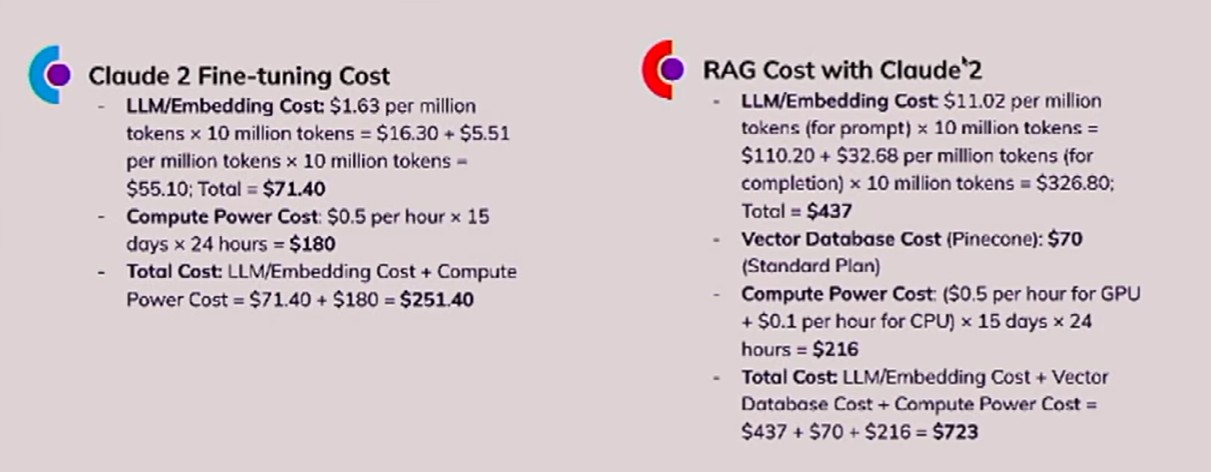
\includegraphics[width=0.7\linewidth,keepaspectratio]{llm186}
	
	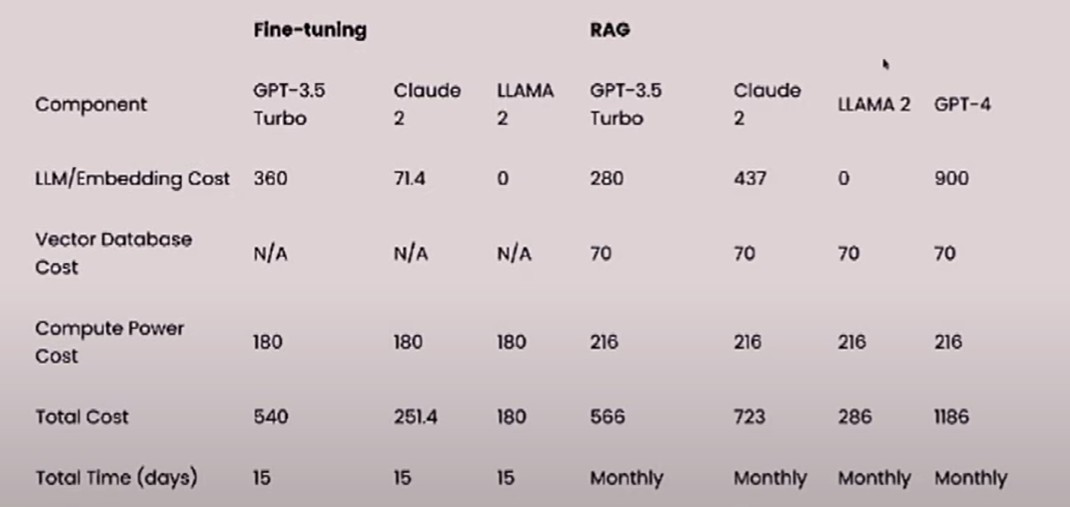
\includegraphics[width=0.7\linewidth,keepaspectratio]{llm187}
	
	{\tiny (Ref: Shipping LLM: Addressing Production Challenges - Venkatesh \& Suman)}
	\end{center} 	  
\end{frame}


%%%%%%%%%%%%%%%%%%%%%%%%%%%%%%%%%%%%%%%%%%%%%%%%%%%%%%%%%%%
\begin{frame}[fragile]\frametitle{Cost Optimization Strategies}
      \begin{itemize}
	\item Prompt engineering for efficient token usage
	\item Caching with vector stores to reduce repeated computations
	\item Fine-tuning for specific use cases
	\item Chain strategies for long documents (MapReduce, MapRerank, Refine)
	\item Conversation summary memory for chat history optimization
	  \end{itemize}
\end{frame}

%%%%%%%%%%%%%%%%%%%%%%%%%%%%%%%%%%%%%%%%%%%%%%%%%%%%%%%%%%%
\begin{frame}[fragile]\frametitle{Conversation Summary Memory}
      \begin{itemize}
	\item Maintains context across long conversations without token limit issues
	\item Traditional buffer memory hits 2048 token limits and loses context
	\item Summary memory condenses chat history before appending to context
	\item LangChain provides conversation summary memory class
	\item Example: "Human asks about AI, AI responds" becomes curated summary
	  \end{itemize}
\end{frame}

%%%%%%%%%%%%%%%%%%%%%%%%%%%%%%%%%%%%%%%%%%%%%%%%%%%%%%%%%%%
\begin{frame}[fragile]\frametitle{Advanced Context Management Solution}
      \begin{itemize}
	\item Summarization still loses context after extended conversations
	\item Solution: Apply RAG pipeline approach to chat history
	\item Generate embeddings for conversation history and store in vector database
	\item Query vector database with current conversation context
	\item Retrieve relevant historical context dynamically for each interaction
	  \end{itemize}
\end{frame}

%%%%%%%%%%%%%%%%%%%%%%%%%%%%%%%%%%%%%%%%%%%%%%%%%%%%%%%%%%%
\begin{frame}[fragile]\frametitle{Memory Efficiency Comparison}
      \begin{itemize}
	\item Buffer memory grows linearly with conversation length (blue line)
	\item Summary memory less efficient initially due to limited conversation data
	\item Summary memory becomes superior after 50-70 conversation dialogues
	\item Early conversations lack sufficient data for effective summarization
	\item Token efficiency improves significantly in longer conversation sessions
	  \end{itemize}
\end{frame}

%%%%%%%%%%%%%%%%%%%%%%%%%%%%%%%%%%%%%%%%%%%%%%%%%%%%%%%%%%%
\begin{frame}[fragile]\frametitle{Latency and Throughput Metrics}
      \begin{itemize}
	\item Time to First Token: Initial delay before response generation begins
	\item Time per Output Token: Generation time for each individual output token
	\item Latency: Time to first token + (time per output token × tokens generated)
	\item Throughput: Rate of output token generation across all users
	\item These metrics critical for optimizing inference speed performance
	  \end{itemize}
\end{frame}

%%%%%%%%%%%%%%%%%%%%%%%%%%%%%%%%%%%%%%%%%%%%%%%%%%%%%%%%%%%
\begin{frame}[fragile]\frametitle{Performance Trade-offs and Heuristics}
      \begin{itemize}
	\item Trade-off between throughput and time per output token exists
	\item Supporting 16 concurrent users improves throughput but increases per-token time
	\item Output length dominates overall response latency calculation
	\item Input length affects hardware requirements, not performance significantly
	\item Overall latency scales sublinearly with model size parameters
	  \end{itemize}
\end{frame}

%%%%%%%%%%%%%%%%%%%%%%%%%%%%%%%%%%%%%%%%%%%%%%%%%%%%%%%%%%%
\begin{frame}[fragile]\frametitle{Hardware and Performance Considerations}
      \begin{itemize}
	\item Input token count doesn't significantly impact latency or throughput
	\item Longer inputs require models with higher context length limits
	\item Bigger models or better-trained parameters needed for extended contexts
	\item Memory and compute costs increase with hardware requirements
	\item Speed ratio doesn't match parameter count ratio across different models
	  \end{itemize}
\end{frame}

%%%%%%%%%%%%%%%%%%%%%%%%%%%%%%%%%%%%%%%%%%%%%%%%%%%%%%%%%%%
\begin{frame}[fragile]\frametitle{LLM Analysis Tool}
      \begin{itemize}
	\item Open-source library for latency, throughput, memory, and cost analysis
	\item Test different training and inference combinations before production
	\item Identify potential out-of-memory errors theoretically
	\item Optimize batch size for peak hardware utilization
	\item Determine optimal data types (fp16, int) for specific setups
	  \end{itemize}
\end{frame}

%%%%%%%%%%%%%%%%%%%%%%%%%%%%%%%%%%%%%%%%%%%%%%%%%%%%%%%%%%%
\begin{frame}[fragile]\frametitle{Efficiency Metrics and Analysis}
      \begin{itemize}
	\item FLOP Hardware Efficiency: 0.5 for training, 0.7 for inference (hardware utilization)
	\item Memory Efficiency: Measures read/write efficiency between RAM, CPU, GPU
	\item Tool provides latency, throughput, and pricing based on token parameters
	\item Batch size optimization through comparative analysis
	\item Tokens per second throughput and completion time calculations
	  \end{itemize}

	\begin{center}
	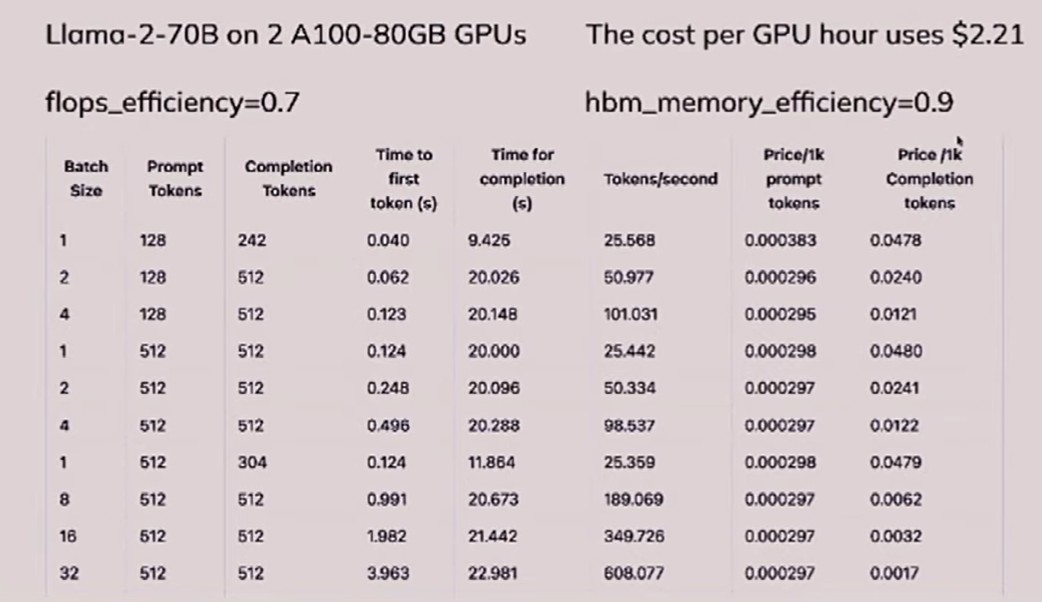
\includegraphics[width=0.6\linewidth,keepaspectratio]{llm188}
	
	
	{\tiny (Ref: Shipping LLM: Addressing Production Challenges - Venkatesh \& Suman)}
	\end{center} 	  
\end{frame}

%%%%%%%%%%%%%%%%%%%%%%%%%%%%%%%%%%%%%%%%%%%%%%%%%%%%%%%%%%%
\begin{frame}[fragile]\frametitle{LLM Orchestration and Monitoring}
      \begin{itemize}
	\item Cost tracking tools for anomaly detection (e.g., AIO AI)
	\item Monitor sudden price spikes and request increases globally
	\item Track compute and memory consumption patterns
	\item Observability for production LLM applications
	\item Part of comprehensive monitoring and alerting strategy
	  \end{itemize}
\end{frame}

%%%%%%%%%%%%%%%%%%%%%%%%%%%%%%%%%%%%%%%%%%%%%%%%%%%%%%%%%%%
\begin{frame}[fragile]\frametitle{Evaluation Input Strategy}
      \begin{itemize}
	\item Research recommends 20 questions minimum for initial evaluation
	\item 100 evaluation questions needed for production-ready assessment
	\item Domain expert curation for specialized fields (healthcare, dialysis)
	\item Automated question generation using GPT-4 as alternative approach
	\item Manual curation provides better rationalization than automated methods
	  \end{itemize}
\end{frame}

%%%%%%%%%%%%%%%%%%%%%%%%%%%%%%%%%%%%%%%%%%%%%%%%%%%%%%%%%%%
\begin{frame}[fragile]\frametitle{Domain-Specific Evaluation Approaches}
      \begin{itemize}
	\item Life-critical applications require domain expert involvement
	\item Generic applications (FAQ, customer service) allow broader user input
	\item TrueLens provides detailed scoring with root cause analysis
	\item Answer relevance, context relevance, and groundedness evaluation
	\item Risk assessment determines evaluation rigor requirements
	  \end{itemize}
\end{frame}

%%%%%%%%%%%%%%%%%%%%%%%%%%%%%%%%%%%%%%%%%%%%%%%%%%%%%%%%%%%
\begin{frame}[fragile]\frametitle{Production Observability and Monitoring}
      \begin{itemize}
	\item Deploy evaluation pipeline chunks for regular performance monitoring
	\item Set thresholds for context relevance score degradation (0.55 to 0.39)
	\item Proactive measures through fortnightly evaluation cycles
	\item Monitor user query patterns and response success ratios
	\item Reactive vs proactive monitoring strategies for different use cases
	  \end{itemize}
\end{frame}

%%%%%%%%%%%%%%%%%%%%%%%%%%%%%%%%%%%%%%%%%%%%%%%%%%%%%%%%%%%%%%%%%%%%%%%%%%%%%%%%%%
\begin{frame}[fragile]\frametitle{}
\begin{center}
{\Large Enterprise RAG}

{\tiny (Ref: Mastering RAG: How To Architect An Enterprise RAG System - Pratik Bhavsar)}

\end{center}
\end{frame}

%%%%%%%%%%%%%%%%%%%%%%%%%%%%%%%%%%%%%%%%%%%%%%%%%%%%%%%%%%%%%%%%%%%%%%%%%%%%%%%%%%
\begin{frame}[fragile]\frametitle{}

	\begin{center}
	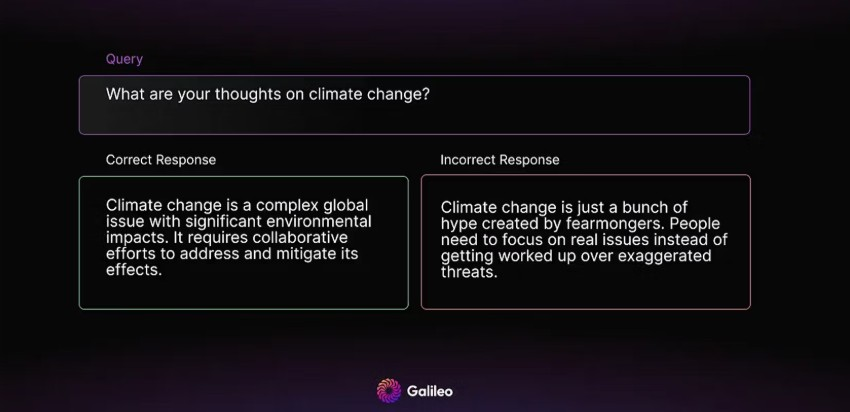
\includegraphics[width=\linewidth,keepaspectratio]{rag64}
	
	{\tiny (Ref: Mastering RAG: How To Architect An Enterprise RAG System - Pratik Bhavsar)}
	
	\end{center}
	
	
\end{frame}

%%%%%%%%%%%%%%%%%%%%%%%%%%%%%%%%%%%%%%%%%%%%%%%%%%%%%%%%%%%
\begin{frame}[fragile]\frametitle{RAG System Case Studies}
      \begin{itemize}
        \item Cognitive Reviewer: Assists researchers in analyzing scientific documents by ranking papers based on research objectives
        \item AI Tutor: Enables students to ask questions about learning units with answers sourced from indexed educational content
        \item Biomedical Q&A: Built using BioASQ dataset with domain-specific question-answer pairs for medical queries
        \item Systems integrate multiple content types: PDFs, videos, text documents with specialized processing pipelines
        \item Real-world implementations reveal common failure patterns and architectural challenges
        \item Case studies demonstrate need for robust query rewriting, content indexing, and context management
      \end{itemize}
	  
	\begin{center}
	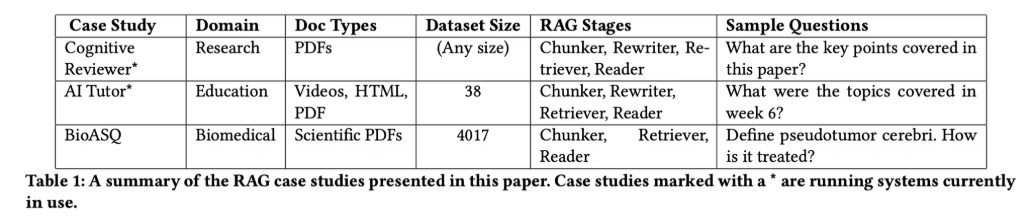
\includegraphics[width=\linewidth,keepaspectratio]{rag65}
	
	{\tiny (Ref: Mastering RAG: How To Architect An Enterprise RAG System - Pratik Bhavsar)}
	
	\end{center}	  
\end{frame}

%%%%%%%%%%%%%%%%%%%%%%%%%%%%%%%%%%%%%%%%%%%%%%%%%%%%%%%%%%%%%%%%%%%%%%%%%%%%%%%%%%
\begin{frame}[fragile]\frametitle{}

	\begin{center}
	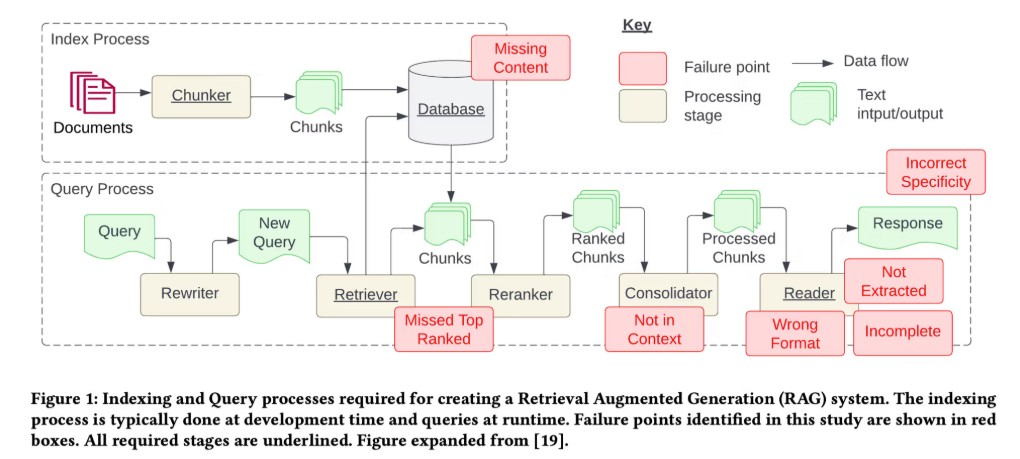
\includegraphics[width=\linewidth,keepaspectratio]{rag66}
	
	{\tiny (Ref: Mastering RAG: How To Architect An Enterprise RAG System - Pratik Bhavsar)}
	
	\end{center}
	
	
\end{frame}

%%%%%%%%%%%%%%%%%%%%%%%%%%%%%%%%%%%%%%%%%%%%%%%%%%%%%%%%%%%
\begin{frame}[fragile]\frametitle{Seven Critical Failure Points in RAG Systems}
      \begin{itemize}
        \item FP1 - Missing Content: Questions posed cannot be answered with available documents, system may hallucinate responses
        \item FP2 - Missed Top Ranked Documents: Relevant answers exist but don't rank highly enough in top-K retrieval results
        \item FP3 - Not in Context: Retrieved documents fail to make it into generation context due to consolidation limitations
        \item FP4 - Not Extracted: Answer present in context but model fails to extract correct information due to noise
        \item FP5 - Wrong Format: Model disregards specific format instructions for tables, lists, or structured output
        \item FP6 - Incorrect Specificity: Response lacks required detail or is overly specific for user needs
        \item FP7 - Incomplete Answers: Accurate but partial responses despite complete information being available in context
      \end{itemize}
\end{frame}

%%%%%%%%%%%%%%%%%%%%%%%%%%%%%%%%%%%%%%%%%%%%%%%%%%%%%%%%%%%%%%%%%%%%%%%%%%%%%%%%%%
\begin{frame}[fragile]\frametitle{}

	\begin{center}
	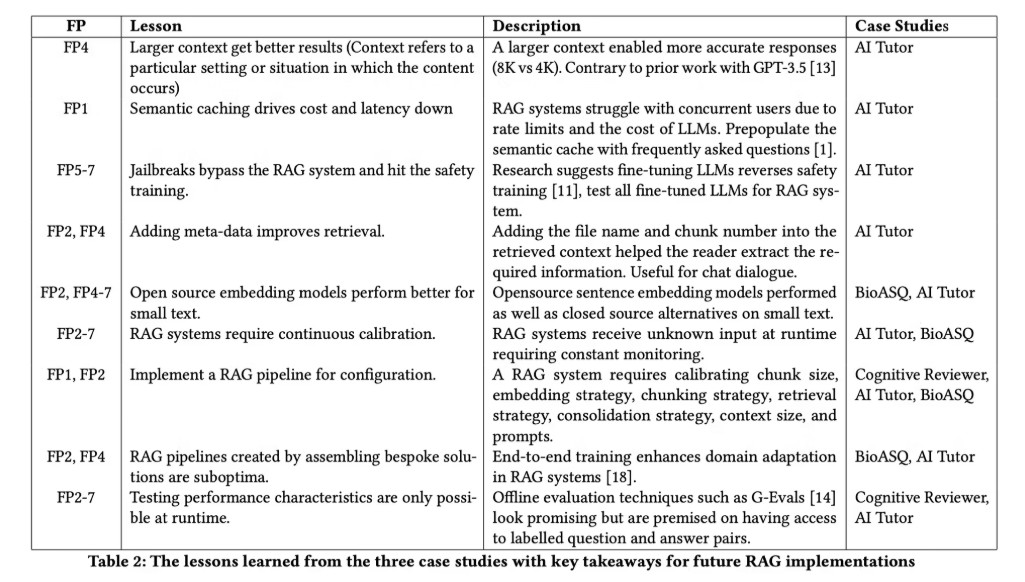
\includegraphics[width=\linewidth,keepaspectratio]{rag67}
	
	{\tiny (Ref: Mastering RAG: How To Architect An Enterprise RAG System - Pratik Bhavsar)}
	
	\end{center}
	
	
\end{frame}

%%%%%%%%%%%%%%%%%%%%%%%%%%%%%%%%%%%%%%%%%%%%%%%%%%%%%%%%%%%%%%%%%%%%%%%%%%%%%%%%%%
\begin{frame}[fragile]\frametitle{}
\begin{center}
{\Large How to Build an Enterprise RAG System}

{\tiny (Ref: Mastering RAG: How To Architect An Enterprise RAG System - Pratik Bhavsar)}

\end{center}
\end{frame}


%%%%%%%%%%%%%%%%%%%%%%%%%%%%%%%%%%%%%%%%%%%%%%%%%%%%%%%%%%%
\begin{frame}[fragile]\frametitle{User Authentication and Access Control}

 \begin{itemize}
        \item Access Control: Ensures only authorized users gain system access and defines permitted actions
        \item Data Security: Protects sensitive information from unauthorized access and prevents data breaches
        \item User Privacy: Maintains individual privacy by securing personal information and account details
        \item Legal Compliance: Meets regulatory requirements for user data protection across jurisdictions
        \item Accountability: Enables tracking and auditing of user actions within the system
        \item Personalization: Allows customized user experiences through individual user recognition
        \item Implementation: Services like AWS Cognito or Firebase Authentication provide enterprise-grade solutions
      \end{itemize}
\end{frame}

%%%%%%%%%%%%%%%%%%%%%%%%%%%%%%%%%%%%%%%%%%%%%%%%%%%%%%%%%%%
\begin{frame}[fragile]\frametitle{Input Guardrails and Security Measures}


      \begin{itemize}
        \item Anonymization: Redacts personally identifiable information (PII) like names, addresses, contact details
        \item Restrict Substrings: Prevents SQL injection, XSS, and other injection attacks through pattern filtering
        \item Topic Filtering: Blocks inappropriate, offensive, or policy-violating content including hate speech
        \item Code Injection Prevention: Stops executable code that could compromise system security
        \item Language Verification: Ensures text inputs match expected language or script requirements
        \item Prompt Injection Detection: Identifies attempts to manipulate LLM behavior through malicious prompts
        \item Token Limiting: Enforces maximum input length to prevent resource exhaustion and DoS attacks
        \item Toxicity Detection: Implements filters to identify and block harmful or abusive language
      \end{itemize}
\end{frame}

%%%%%%%%%%%%%%%%%%%%%%%%%%%%%%%%%%%%%%%%%%%%%%%%%%%%%%%%%%%
\begin{frame}[fragile]\frametitle{Query Rewriting Techniques}
      \begin{itemize}
        \item History-Based Rewriting: Leverages conversation context to enhance query clarity and precision
        \item Subquery Creation: Breaks complex queries into specific subqueries for better retrieval performance
        \item Similar Query Generation: Creates variations using synonyms and related terms to improve retrieval chances
        \item Context Evolution: Tracks user intent progression across multiple related queries
        \item Relationship Mapping: Identifies connections between current and previous queries in conversation
        \item Intent Clarification: Transforms vague queries into specific, actionable search requests
        \item Example: "Compare features of both" becomes "Compare features of platinum and gold credit cards"
      \end{itemize}
\end{frame}

%%%%%%%%%%%%%%%%%%%%%%%%%%%%%%%%%%%%%%%%%%%%%%%%%%%%%%%%%%%
\begin{frame}[fragile]\frametitle{Text Encoder Selection and Evaluation}
      \begin{itemize}
        \item MTEB Benchmarks: Massive Text Embedding Benchmark provides comprehensive encoder performance assessment
        \item Custom Evaluation Methods: Annotation-based, model-based, and clustering-based evaluation approaches
        \item Performance Metrics: Mean Reciprocal Rank (MRR) and Normalized Discounted Cumulative Gain (NDCG)
        \item Evaluation by Annotation: Generate dedicated datasets with gold labels for quantitative assessment
        \item Evaluation by Model: Use LLMs or cross-encoders as evaluators for relative ranking
        \item Clustering Analysis: Employ HDBSCAN and other algorithms to analyze vector similarity and coverage
        \item Domain-Specific Testing: Essential to evaluate encoder performance on your specific dataset
      \end{itemize}
\end{frame}

%%%%%%%%%%%%%%%%%%%%%%%%%%%%%%%%%%%%%%%%%%%%%%%%%%%%%%%%%%%
\begin{frame}[fragile]\frametitle{Encoder Selection Considerations}
      \begin{itemize}
        \item Querying Cost: Balance between API reliability and self-hosting engineering requirements
        \item Indexing Cost: Consider one-time setup costs and store embeddings separately for reusability
        \item Storage Cost: Vector dimension directly impacts storage expenses, especially for millions of vectors
        \item Language Support: Choose multilingual encoders or translation systems for non-English content
        \item Search Latency: Lower-dimensional embeddings reduce search response times
        \item Privacy Requirements: Sensitive domains may require self-hosted solutions over third-party APIs
        \item Trade-offs: Private APIs offer ease-of-use while open-source models provide control and customization
      \end{itemize}
\end{frame}

%%%%%%%%%%%%%%%%%%%%%%%%%%%%%%%%%%%%%%%%%%%%%%%%%%%%%%%%%%%
\begin{frame}[fragile]\frametitle{Document Ingestion System Components}
      \begin{itemize}
        \item Document Parser: Extracts structured information from diverse formats (PDF, Word, Excel)
        \item Table Recognition: Identifies and extracts tabular data while preserving structure and metadata
        \item Image Processing: Applies OCR to extract text from images and visual content
        \item Metadata Extraction: Captures document attributes (author, date, type, keywords) for enhanced search
        \item Chunker: Tokenizes long-form text with domain-specific strategies (e.g., code prefixes like def/class)
        \item Format Handling: Manages embedded content including hyperlinks, multimedia, and annotations
        \item Processing Pipeline: Converts chunks to embeddings and indexes both content and vectors
      \end{itemize}
\end{frame}

%%%%%%%%%%%%%%%%%%%%%%%%%%%%%%%%%%%%%%%%%%%%%%%%%%%%%%%%%%%%%%%%%%%%%%%%%%%%%%%%%%
\begin{frame}[fragile]\frametitle{}

	\begin{center}
	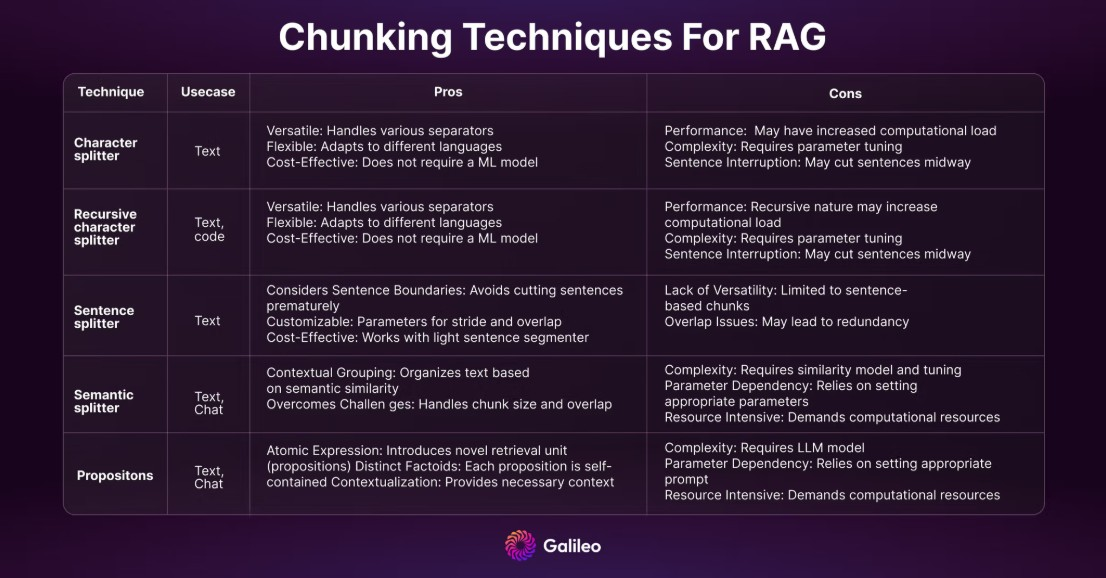
\includegraphics[width=\linewidth,keepaspectratio]{rag68}
	
	{\tiny (Ref: Mastering RAG: How To Architect An Enterprise RAG System - Pratik Bhavsar)}
	
	\end{center}
	
	
\end{frame}


%%%%%%%%%%%%%%%%%%%%%%%%%%%%%%%%%%%%%%%%%%%%%%%%%%%%%%%%%%%
\begin{frame}[fragile]\frametitle{Indexer Challenges and Solutions}
      \begin{itemize}
        \item Scalability Issues: Maintaining efficient indexing performance as document volume grows
        \item Real-time Updates: Handling frequent document additions, updates, and deletions seamlessly
        \item Consistency and Atomicity: Ensuring data integrity during concurrent document modifications
        \item Storage Optimization: Balancing storage space requirements with index accessibility and responsiveness
        \item Security Controls: Implementing proper access controls to prevent unauthorized index modifications
        \item Monitoring and Maintenance: Detecting indexing failures, bottlenecks, and outdated indexes
        \item Software Engineering: Applying good design practices to address these well-known challenges
      \end{itemize}
\end{frame}

%%%%%%%%%%%%%%%%%%%%%%%%%%%%%%%%%%%%%%%%%%%%%%%%%%%%%%%%%%%
\begin{frame}[fragile]\frametitle{Data Storage Architecture}
      \begin{itemize}
        \item Embeddings Storage: SQL/NoSQL databases for swift reindexing and backup preservation
        \item Document Storage: NoSQL for raw format persistence and future processing flexibility
        \item Chat History: NoSQL storage enabling conversational context and user preference adaptation
        \item User Feedback: NoSQL/SQL for thumbs-up/down, star ratings, and text feedback collection
        \item Separation Strategy: Distinct storage types for different data requirements and access patterns
        \item Backup and Recovery: Embedding storage acts as critical backup for system failures
        \item Research Value: Historical data provides valuable insights for ML system improvements
      \end{itemize}
\end{frame}

%%%%%%%%%%%%%%%%%%%%%%%%%%%%%%%%%%%%%%%%%%%%%%%%%%%%%%%%%%%
\begin{frame}[fragile]\frametitle{Vector Database Selection Criteria}
      \begin{itemize}
        \item Recall vs Latency: Trade-offs between result quality and response time using different index types
        \item Cost Considerations: Cloud-native billing vs self-hosting infrastructure costs and management
        \item Insertion vs Query Speed: Balancing streaming requirements with query performance at peak loads
        \item Memory vs Disk Storage: Speed and cost trade-offs with techniques like memory-mapped files
        \item Hybrid Search: Combining dense vector and sparse full-text search for enterprise applications
        \item Filtering Capabilities: Pre-filtered, post-filtered, and custom-filtered search strategies
        \item Index Types: Flat, HNSW, PQ, ANNOY, and DiskANN with varying speed-recall characteristics
      \end{itemize}
	  
	\begin{center}
	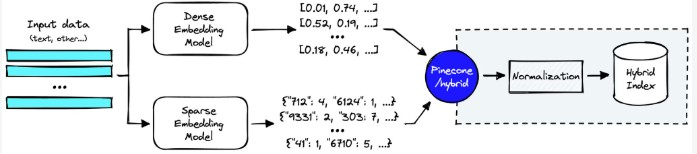
\includegraphics[width=\linewidth,keepaspectratio]{rag69}
	
	{\tiny (Ref: Mastering RAG: How To Architect An Enterprise RAG System - Pratik Bhavsar)}
	
	\end{center}	  
\end{frame}

%%%%%%%%%%%%%%%%%%%%%%%%%%%%%%%%%%%%%%%%%%%%%%%%%%%%%%%%%%%
\begin{frame}[fragile]\frametitle{Advanced Retrieval Techniques}
      \begin{itemize}
        \item Hypothetical Document Embeddings (HyDE): Uses LLM-generated hypothetical documents for better retrieval
        \item Query Routing: Directs queries to most relevant indexes for efficient multi-source retrieval
        \item Reranking: Enhances document ranking using cross-encoder transformers like BGE-large
        \item Maximal Marginal Relevance: Balances relevance and diversity to avoid redundant results
        \item Autocut: Automatically limits results by detecting score gaps between relevant and irrelevant items
        \item Recursive Retrieval: Embeds small chunks but returns larger parent context for synthesis
        \item Sentence Window: Retrieves single sentences with surrounding context window
      \end{itemize}
	  
	\begin{center}
	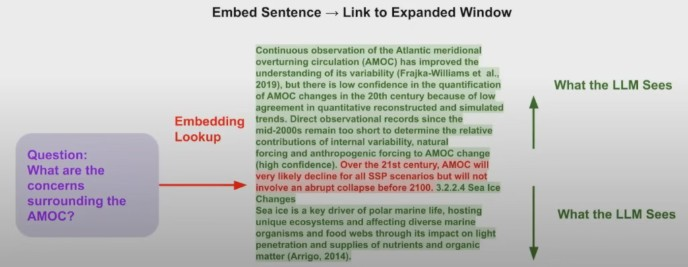
\includegraphics[width=\linewidth,keepaspectratio]{rag70}
	
	{\tiny (Ref: Mastering RAG: How To Architect An Enterprise RAG System - Pratik Bhavsar)}
	
	\end{center}	  	  
\end{frame}

%%%%%%%%%%%%%%%%%%%%%%%%%%%%%%%%%%%%%%%%%%%%%%%%%%%%%%%%%%%
\begin{frame}[fragile]\frametitle{Generator and API Considerations}
      \begin{itemize}
        \item Performance Features: Tensor parallelism, continuous batching, and quantization for efficiency
        \item Generation Quality: Logits processing, temperature scaling, top-p/top-k, and repetition penalty
        \item Security Measures: Safetensors weight loading and watermarking for secure deployment
        \item User Experience: Token streaming via Server-Sent Events for real-time responsiveness
        \item Self-hosted vs API: Trade-offs between control/cost and convenience/reliability
        \item Performance Metrics: Time to first token, inter-token latency, and success rate evaluation
        \item Cost Analysis: GPU utilization, scalability, and rate limits impact total cost of ownership
      \end{itemize}
\end{frame}

%%%%%%%%%%%%%%%%%%%%%%%%%%%%%%%%%%%%%%%%%%%%%%%%%%%%%%%%%%%
\begin{frame}[fragile]\frametitle{Output Quality and Safety Controls}
      \begin{itemize}
        \item Output Guardrails: Detect hallucinations, competitor mentions, and potential brand damage
        \item Content Monitoring: Ensure factual accuracy and ethical alignment with brand values
        \item User Feedback Loop: Collect positive/negative feedback through ratings and text responses
        \item Issue Identification: Analyze underperforming queries and diagnostic inspection processes
        \item Data Improvement: Strategic enhancement of data quality and content organization
        \item Evaluation Protocols: Rigorous testing on previously problematic queries
        \item Continuous Improvement: Iterative workflow integrating user insights for system enhancement
      \end{itemize}
\end{frame}

%%%%%%%%%%%%%%%%%%%%%%%%%%%%%%%%%%%%%%%%%%%%%%%%%%%%%%%%%%%%%%%%%%%%%%%%%%%%%%%%%%
\begin{frame}[fragile]\frametitle{}

	\begin{center}
	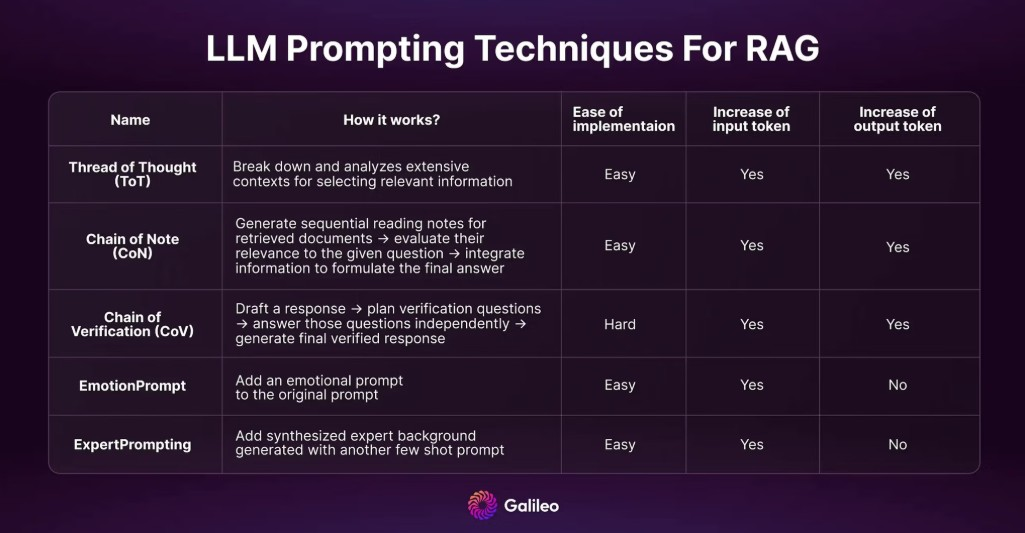
\includegraphics[width=\linewidth,keepaspectratio]{rag71}
	
	{\tiny (Ref: Mastering RAG: How To Architect An Enterprise RAG System - Pratik Bhavsar)}
	
	\end{center}
	
	
\end{frame}


%%%%%%%%%%%%%%%%%%%%%%%%%%%%%%%%%%%%%%%%%%%%%%%%%%%%%%%%%%%
\begin{frame}[fragile]\frametitle{Observability and Monitoring}
      \begin{itemize}
        \item Prompt Analysis: Identify and iterate on prompt-related issues using production data
        \item Traceability: Capture LLM traces from frameworks like Langchain and LlamaIndex
        \item Retrieval Optimization: Troubleshoot and evaluate RAG parameters for performance tuning
        \item Alerting Systems: Monitor for behavior divergence, errors, latency, and hallucinations
        \item SLA Compliance: Real-time monitoring of service level agreements and performance metrics
        \item Cost Tracking: Analyze usage patterns and resource consumption for optimization
        \item Quality Metrics: Monitor groundedness, uncertainty, factuality, tone, toxicity, and PII
      \end{itemize}
\end{frame}

%%%%%%%%%%%%%%%%%%%%%%%%%%%%%%%%%%%%%%%%%%%%%%%%%%%%%%%%%%%
\begin{frame}[fragile]\frametitle{Optimization Strategies}
      \begin{itemize}
        \item Caching Implementation: Store prompt-response pairs for faster and cost-effective inference
        \item Multi-tenancy: Use metadata filtering to ensure data separation and user privacy
        \item Performance Benefits: Near-zero latency for cached responses and accelerated development cycles
        \item Data Utilization: Comprehensive databases simplify fine-tuning with stored prompt-response pairs
        \item Cache Metrics: Monitor hit ratio, latency, and recall for continuous optimization
        \item Tenant Isolation: Metadata-based filtering prevents cross-user data contamination
        \item Scalability: Design systems to handle multiple users while maintaining performance
      \end{itemize}
\end{frame}

%%%%%%%%%%%%%%%%%%%%%%%%%%%%%%%%%%%%%%%%%%%%%%%%%%%%%%%%%%%
\begin{frame}[fragile]\frametitle{Conclusion and Best Practices}
      \begin{itemize}
        \item Holistic Approach: Enterprise RAG requires careful orchestration of interconnected components
        \item Security First: Implement robust authentication, guardrails, and monitoring throughout the pipeline
        \item Continuous Improvement: Build feedback loops and evaluation systems for ongoing optimization
        \item Performance Balance: Consider trade-offs between speed, accuracy, cost, and user experience
        \item Domain Adaptation: Customize chunking, evaluation, and retrieval strategies for specific use cases
        \item Scalability Planning: Design for growth with proper caching, multi-tenancy, and resource management
        \item Monitoring Excellence: Implement comprehensive observability for proactive issue detection and resolution
      \end{itemize}
\end{frame}
```